%%%%%%%%%%%%%%%%%%%%%%%%%%%%%%%%%%%%%%%%%%%%%%%
%%% Template for lab reports used at BIT modified from STIMA
%%% Author: Charlie Li
%%%%%%%%%%%%%%%%%%%%%%%%%%%%%%%%%%%%%%%%%%%%%%%

%%%%%%%%%%%%%%%%%%%%%%%%%%%%%% Sets the document class for the document
% Openany is added to remove the book style of starting every new chapter on an odd page (not needed for reports)
\documentclass[12pt,openany,a4paper]{book}
%%%%%%%%%%%%%%%%%%%%%%%%%%%%%% Loading packages that alter the style
\usepackage[]{graphicx}
\usepackage[]{color}
\usepackage{alltt}
\usepackage[T1]{fontenc}
\usepackage[utf8]{inputenc}
\usepackage{polski}
% \usepackage[polish]{babel}
% Math
\usepackage{amsmath}
\usepackage{amssymb}
\usepackage{physics}
% Fonts
\renewcommand{\rmdefault}{ptm}
\renewcommand{\sfdefault}{phv}


\setcounter{secnumdepth}{3}
\setcounter{tocdepth}{3}
\setlength{\parskip}{\smallskipamount}
\setlength{\parindent}{12pt}
\usepackage{indentfirst}

% Set page margins
\usepackage[top=50pt,bottom=60pt,left=70pt,right=70pt]{geometry}
\usepackage{subcaption}
% Package used for placeholder text
\usepackage{booktabs}
\usepackage{multirow}
% Prevents LaTeX from filling out a page to the bottom
\raggedbottom{}

% Adding both languages
% \usepackage[english]{babel}

% All page numbers positioned at the bottom of the page
\usepackage{fancyhdr}
\fancyhf{} % clear all header and footers
\fancyfoot[C]{\thepage}
%\fancyhead[L]{{\selectfont \leftmark}}
\renewcommand{\headrulewidth}{0pt} % remove the header rule
\pagestyle{fancy}

% Changes the style of chapter headings
\usepackage{titlesec}
\titleformat{\chapter}
{\normalfont\LARGE\bfseries}{\thechapter.}{1em}{}
% Change distance between chapter header and text
\titlespacing{\chapter}{0pt}{40pt}{2\baselineskip}

% Adds table captions above the table per default
\usepackage{float}
\floatstyle{plaintop}
\restylefloat{table}

% Adds space between caption and table
\usepackage[tableposition=top]{caption}

% add cc license
% \usepackage[
% type={CC},
% modifier={by-nc-sa},
% version={4.0},
% ]{doclicense}

% Adds hyperlinks to references and ToC
\usepackage{hyperref}
% \usepackage[backref=page]{hyperref} % hyperlinks
% \renewcommand*{\backref}[1]{}
% \renewcommand*{\backrefalt}[4]{{\footnotesize [%
% 		\ifcase #1 Not cited.%
% 		\or Cited on page~#2%
% 		\else Cited on pages #2%
% 		\fi%
% 		]}}
\usepackage[capitalise]{cleveref}

% Uncomment the line below this block to set all hyperlink color to black
\hypersetup{
	colorlinks,
	linkcolor={blue},
	citecolor={green!90!black},
	urlcolor={red!70!black}
}
%\hypersetup{hidelinks,linkcolor = black} % Changes the link color to black and hides the hideous red border that usually is created

% Set specific color for hyperref
\usepackage{xcolor}


% tcolorbox; Notice! add "-shell-escape" to the compile command
\usepackage{tcolorbox}

% If multiple images are to be added, a folder (path) with all the images can be added here 
% \graphicspath{ {Figures/} }

% Separates the first part of the report/thesis in Roman numerals
\frontmatter
\patchcmd{\chapter}{\thispagestyle{plain}}{\thispagestyle{fancy}}{}{}{}
% Uncomment to stop the new chapter start at a new page
\usepackage{etoolbox}
\makeatletter
\patchcmd{\chapter}{\if@openright\cleardoublepage\else\clearpage\fi}{}{}{}
\patchcmd{\section}{\if@openright\cleardoublepage\else\clearpage\fi}{}{}{}
\makeatother


\usepackage{bpchem}
\usepackage{epstopdf}
\usepackage[
    backend=biber,
	% babel = other,
    style=numeric,
	sorting=none
  ]{biblatex}
\addbibresource{C:/texlive/Bibtex/AlGaAsSb.bib}
\usepackage{siunitx}
\usepackage{caption}
% \addbibresource{ref.bib}
%%%%%%%%%%%%%%%%%%%%%%%%%%%%%% Starts the document
\begin{document}
	

	
	%%%%% Adds the title page
	\begin{titlepage}
		\clearpage\thispagestyle{empty}
		\centering
		\vspace{1cm}
		
		% Titles
		% Information about the University
		{\
			\textsc{Projektowanie Struktur Półprzewodnikowych}
		}
		\vspace{2.5cm}
		
		\rule{\linewidth}{2mm} \\[0.8cm]
		{ \LARGE \sc Sprawozdanie}\\[0.55cm]
		\rule{\linewidth}{0.6mm} \\[3.4cm]
		
		\hspace{2cm}
		\begin{tabular}{l p{5cm}}
			\textbf{Imię} & Jakub Pawłowski \\[10pt]
			\textbf{Numer albumu} & \texttt{250193} \\[10pt]
			\textbf{Kierunek} & \texttt{Inżynieria Kwantowa} \\[10pt]
			\textbf{Rok/Semestr} & Semestr letni 2020/2021 \\[10pt]
			\textbf{Materiał} & \BPChem{AlGaAsSb} \\[10pt]
			\textbf{Data} & \today \\            
		\end{tabular}
		
		
		\vfill
		% \centering
\includegraphics{Figures/pwr.eps}
		\centering 
\includegraphics[width = \linewidth]{Figures/pwr.png}
		\vspace{0.5cm}
		
		
		
		
		\pagebreak
		
	\end{titlepage}
	%% Uncomment for title page print two pages per sheet
	%\shipout\null
	
	% Comment the following two lines to remove abstract 
	% \chapter*{\makebox[\linewidth]{Abstract}}
	% \addcontentsline{toc}{chapter}{Abstract}
	% This is a template for Projects/Report/Proposals at BIT. ~\lipsum[5]
	
	% \vspace{0.5cm}
	% \noindent\textbf{Keywords}: 
	% \LaTeX, BIT
	% \clearpage
	
	% Adds a table of contents keep the link black
	\let\cleardoublepage\clearpage
	{\hypersetup{linkcolor=black}
		% or \hypersetup{linkcolor=black}, if the colorlinks=true option of hyperref is used
		\tableofcontents{}
		\listoffigures{}
	}
	
	%%%%%%%%%%%%%%%%%%%%%%%%%%%%%%%%%%%%%%%%%%%%%%%%%%%%%%%%%%%%%%%%%%%%%%%%%%%%%%%%%%%%%%%%%%%%
	%%%%%%%%%%%%%%%%%%%%%%%%%%%%%%%%%%%%%%%%%%%%%%%%%%%%%%%%%%%%%%%%%%%%%%%%%%%%%%%%%%%%%%%%%%%%
	%%%%% Text body starts here!
	\mainmatter{}
	
	
	\chapter{Opis systemu materiałowego}\label{chapt:opis}
	
	Badanym materiałem jest czteroskładnikowy stop \BPChem{AlGaAsSb}. Znajduję on zastosowanie m.in. w budowie
	laserów na heterostrukturach~\autocite{Morosini1993}, kaskadowych ogniw słonecznych~\autocite{Timmons1981} oraz
	w charakterze szerokopasmowego źródła światła wysokiej mocy, na zakresie spektralnym \SI{2.2}{\micro\metre} do \SI{2.5}{\micro\metre},
	opartego na studni kwantowej~\autocite{Wootten2014}.\\

	Składa się on z 4 materiałów binarnych, związków III-V tj.:
	\begin{itemize}
		\item \BPChem{AlAs}
		\item \BPChem{AlSb}
		\item \BPChem{GaAs}
		\item \BPChem{GaSb}
	\end{itemize} 
	Informacje o materiałach binarnych posłużą nam do wyznaczenia podstawowych parametrów materiałowych.
	Związki III-V w rozpatrywanym stopie czteroskładnikowym mieszają się, tworząc stopy trójskładnikowe.
	Są to:
	\begin{itemize}
		\item \BPChem{AlGaAs}
		\item \BPChem{AlGaSb}
		\item \BPChem{AlAsSb}
		\item \BPChem{GaAsSb}
	\end{itemize}
	
	\section{Zastosowania materiałów binarnych}
	\BPChem{AlAs}, \BPChem{GaAs}, \BPChem{AlSb} oraz \BPChem{GaSb} tworzą kryształy o strukturze blendy cynkowej (stałe sieciowe odpowiednio \SI{5.6611}{\angstrom}, \SI{5.6533}{\angstrom}, \SI{6.1355}{\angstrom} oraz \SI{6.0959}{\angstrom}) i grupie przestrzennej
	\(F\overline{4}3m\). Parametry materiałowe opisujące te związki można znaleźć w~\textcite{Adachi1985,Vurgaftman2001,Adachi1989,Adachi2017}.


	\BPChem{AlSb} jest półprzewodnikiem grupy III-V o przerwie energetycznej \SI{1.6}{\electronvolt}. Ze względu na możliwość
	hodowli dużych, pojedynczych kryształów o ruchliwości elektronów do \SI{350}{\centi\metre^2\per\volt\second} materiał ten jest
	wykorzystywany jako detektor fotonów~\autocite{Seeger1991}.

	\BPChem{GaAs} jest półprzewodnikiem grupy III-V o przerwie energetycznej \SI{1.441}{\electronvolt}. Jest to jeden
	z najbardziej popularnych półprzewodników. Stosowany zarówno w charakterze emitera promieniowania np. diody LED świecące
	w bliskiej podczerwieni~\autocite{Hall1962} oraz absorbera, umożliwiając konstrukcję bardzo wydajnych ogniw słonecznych,
	zbliżających się do limitu Shockleya–Queissera~\autocite{Wang2013}.

	\BPChem{GaSb} jest półprzewodnikiem grupy III-V o wąskiej przerwie energetycznej \SI{0.67}{\electronvolt}~\autocite{Dubey2006}.
	Materiał ten ma duży potencjał do zastosowań elektro-optycznych w zakresie bliskiej podczerwieni. Homozłącza oparte na \BPChem{GaSb}
	są dobrym kandydatem na szybkie fotodiody lawinowe o niskim szumie~\autocite{Milnes1993}. Ze względu na stałą sieciową zgodną z różnymi
	trój- i czteroskładnikowymi stopami III-V, pokrywającymi szeroki zakres spektralny od \SI{0.8}{\micro \metre} do \SI{4.3}{\micro \metre}
	znajduje on zastosowanie jako substrat do tworzenia źródeł i detektorów~\autocite{Dutta1997}. Wykorzystywany jest również do budowy diód
laserowych oraz fotodetektorów o wysokiej wydajności kwantowej~\autocite{Hildebrand1980,Hildebrand1981}.

\BPChem{AlAs} jest półprzewodnikiem grupy III-V o skośnej przerwie wzbronionej \SI{2.16}{\electronvolt}~\autocite{Bouarissa2009}.
	Materiał ten znajduje zastosowanie jako emiter, np. do budowy stosowanych w spektroskopii kwantowych laserów kaskadowych operujących na zakresie
	spektralnym odpowiadającym częstością \SI{3.4}{\tera\hertz} do \SI{5}{\tera\hertz} co odpowiada bliskiej podczerwieni~\autocite{Schrottke2016}.


\section{Zastosowania stopów trójskładnikowych}
\BPChem{Al\_{x}Ga\_{1-x}As} jest materiałem półprzewodnikowym zbliżonym pod względem stałej sieciowej do \BPChem{GaAs},
jednak o większej przerwie wzbronionej, która zmienia się między \SI{1.42}{\electronvolt} a \SI{2.16}{\electronvolt}.
Dla \(x < 0.4\) przerwa fundamentalna jest prosta. Znajduje on zastosowanie do budowy wydajnych fotodetektorów
opartych na studiach kwantowych i pracujących w zakresie podczerwieni~\autocite{Kock1992a}. W tym materiale zaobserwowane
zostały również nieliniowe efekty optyczne~\autocite{Aitchison1997}.

\BPChem{Al\_{x}Ga\_{1-x}Sb} jest materiałem półprzewodnikowym grupy III-V. Przypomina on \BPChem{Al\_{x}Ga\_{1-x}As} tylko o niższej
przerwie wzbronionej. Znajduje on zastosowanie do budowy fotodetektorów pracujących w podczerwieni~\autocite{Law1981}, w tym do diod lawinowych~\autocite{Hildebrand1980,Hildebrand1981}.


\BPChem{AlAs\_{x}Sb\_{1-x}} jest materiałem półprzewodnikowym grupy III-V. Stosowany jest w charakterze zarówno detektora, do budowy
nisko zaszumionych diód lawinowych~\autocite{Tan2012} oraz emitera, w kwantowych laserach kaskadowych o długości fali ok. \(\lambda = \SI{3.7}{\micro\metre}\)
w temperaturze pokojowej, a więc pracujących w zakresie bliskiej podczerwieni~\autocite{Yang2006}.

\BPChem{GaAs\_{1-x}Sb\_{x}} jest materiałem półprzewodnikowym grupy III-V. Stosowany jest głównie jako
fotodetektor pracujący w bliskiej podczerwieni~\autocite{Sun2002,Li2015}. Innym interesującą aplikacją
tego materiału jest zwiększenie długości fali emitowanej z kropki kwantowej \BPChem{InAs/GaAs}, poprzez
naniesienie jego cienkiej warstwy zmniejszającej odkształcenia w kropce~\autocite{Liu2005}.



Parametry nieliniowości stopów trójskładnikowych mogą zostać znalezione w \textcite{Vurgaftman2001,Linnik2000,Adachi1989,Adachi2017,Mozume2008}.



% \section{test}
	

\chapter{Opis modeli i metod. Własności stopu czteroskładnikowego.}\label{chapt:methods}
\section{Schemat interpolacyjny}\label{sec:interpolation}
W celu znalezienia parametrów stopów trójskładnikowych znając parametry materiałów binarnych
	możemy posłużyć się dobrze znanym schematem interpolacyjnym~\autocite{Adachi1985}. W najprostszym, liniowym
	przybliżeniu parametr \(T\) materiału trójskładnikowego  może zostać wyznaczonych przy pomocy
	parametrów binarnych korzystając ze wzoru:
	\begin{equation}
		T_{A_x B_{1-x}C}(x) = x B_{AC} + (1-x)B_{BC} \equiv a + bx
		\label{eq:linear_interp}
	\end{equation}
	gdzie \(a = B_{BC}\) oraz \(b = B_{AC}-B_{BC}\)
	W praktyce, niektóre parametry materiałowe znacznie odbiegają od
	relacji~\eqref{eq:linear_interp} i wykazują w przybliżeniu kwadratową
	zależność od ułamka molowego \(x\)~\autocite{Adachi2017}:
	\begin{equation}
		T_{A_x B_{1-x}C}(x) = x B_{AC} + (1-x)B_{BC}  - C_{A-B}x(1-x)\equiv a + bx+cx^2
		\label{eq:quadratic}
	\end{equation} 
	gdzie \(a = B_{BC}\), \(b = B_{AC} - B_{BC}+C_{A-B}\) oraz \(c = C_{A-B}\). Parametr \(c\)
	to tzw. bowing parameter czyli parametr nieliniowości. Tym równaniem będziemy się posługiwali
	do wyznaczenia własności stopów trójskładnikowych, w przypadku liniowym podstawiając
	wartość \(0\) za parametr nieliniowości.\\

	W przypadku, gdy interesują nas własności stopu czteroskładnikowego postaci
	\BPChem{A\_{x}B\_{1-x}C\_{y}D\_{1-y}}, a znamy już własności stopów trójskładnikowych
	składających się na ten materiał możemy posłużyć się następującym związkiem~\autocite{Adachi2017}:
	\begin{align}
		Q(x,y) = & \frac{x(1-x)\left[y T_{ABC}(x) + (1-y)T_{ABD}(x)\right]}{
			x(1-x) + y(1-y)} \\
			&+ \frac{y(1-y)\left[x T_{ACD}(y) + (1-x)T_{BCD}(y)\right]}{x(1-x) + y(1-y)}
			\label{eq:quaternary} 
	\end{align}

\section{Parametry materiałów binarnych. Parametry nieliniowości.}\label{sec:binary_params}

Większość wykorzystanych parametrów materiałów binarnych oraz parametrów nieliniowości
pochodzi z pracy przeglądowej~\citetitle{Vurgaftman2001},~\textcite{Vurgaftman2001}, za wyjątkiem mas
efektywnych dziur lekkich, ciężkich oraz odpowiednich parametrów nieliniowości,
które zostały zaczerpnięte z książki~\citetitle{Adachi2009},~\textcite{Adachi2009}.
Parametry materiałów binarnych zostały przedstawione w tabeli~\ref{tab:binary}
\begin{table}[htbp]
	\centering
	\caption{Parametry materiałów binarnych~\autocite{Vurgaftman2001,Adachi2009}}
	  \begin{tabular}{ccccc}
	  \toprule
	  \toprule
	  Parametr & \BPChem{AlAs} & \BPChem{AlSb} &  \BPChem{GaSb} & \BPChem{GaAs}\\
	  \midrule
	  \(E_g^{\Gamma}\)(eV)  &3.099 &2.386 &0.812 &1.519  \\
	  VBO (eV)   & -1.33&-0.41 &-0.03 & -0.80 \\
	  \(\Delta_{\textrm{SO}}\) (eV)  &0.28 &0.676 &0.76 & 0.341 \\
	  \(a_{lc}\) (\AA) &5.6611 &6.1355 & 6.0959& 5.65325\\
	  \(m_e^{\ast}\)    &0.15 & 0.14& 0.039& 0.067 \\
	  \(m_{hh}^{\textrm{DOS}}\)  &0.81 &0.9 &0.37 & 0.55 \\
	  \(m_{lh}^{\textrm{DOS}}\)    &0.16 & 0.13& 0.043& 0.083\\
	\bottomrule
	\bottomrule  
	\end{tabular}%
	\label{tab:binary}%
  \end{table}%

  \begin{table}[htbp]
	\centering
	\caption{Parametry nieliniowości stopów trójskładnikowych~\autocite{Vurgaftman2001,Adachi2009}.
	Brak parametru nieliniowości oznaczony został ``---''.}
	  \begin{tabular}{ccccc}
	  \toprule
	  \toprule
	  Parametr & \BPChem{Al\_{x}Ga\_{1-x}As} & \BPChem{Al\_{x}Ga\_{1-x}Sb} &  \BPChem{AlAs\_{x}Sb\_{1-x}} & \BPChem{GaAs\_{x}Sb\_{1-x}}\\
	  \midrule
	  \(E_g^{\Gamma}\)(eV)  &\(-0.127+1.310x\)& \(-0.044+1.22x\)& 0.8 &1.43  \\
	  VBO (eV)   & --- &--- &-1.71 & -1.06 \\
	  \(\Delta_{\textrm{SO}}\) (eV)  &--- &0.3 &0.15 & 0.6 \\
	  \(a_{lc}\) (\AA) &--- &--- & ---& ---\\
	  \(m_e^{\ast}\)    &--- & ---& ---& \eqref{eq:me_bow} \\
	  \(m_{hh}^{\textrm{DOS}}\)  &---&--- &--- &--- \\
	  \(m_{lh}^{\textrm{DOS}}\)    &--- & ---& ---&---\\
	\bottomrule
	\bottomrule  
	\end{tabular}%
	\label{tab:bowing}%
  \end{table}%
Parametry nieliniowości zostały przedstawione w tabeli~\ref{tab:bowing}. Masa efektywna elektronu
w \BPChem{GaAs\_{x}Sb\_{1-x}} wyrażona jest wzorem~\autocite{Adachi2009}:
\begin{equation}
	m_e^{\ast}(x) = 0.039+0.014x + 0.014x^2
	\label{eq:me_bow}
\end{equation}
\section{Obliczone parametry stopów trójskładnikowych i stopu czteroskładnikowego.}

Schematy interpolacyjne opisane w~\ref{sec:interpolation} zostały zaimplementowane w języku Python.
Wyniki obliczeń przedstawiono na wykresach.\\

\begin{figure}[H]
	\centering
	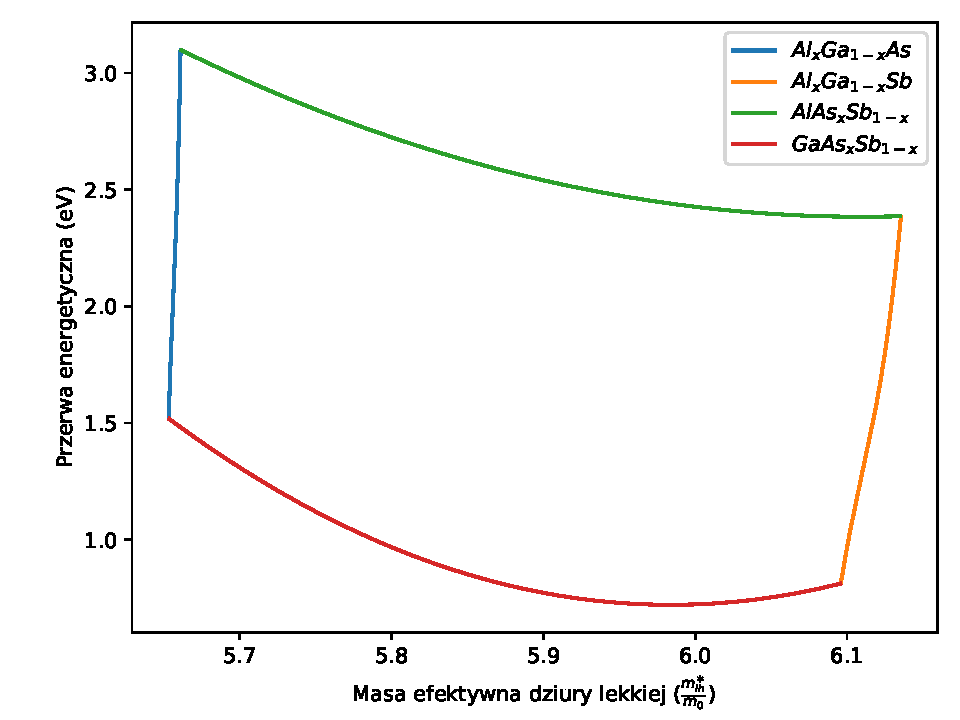
\includegraphics[width = 0.8\linewidth]{Figures/ternary/Eg_alc.pdf}
	\caption{Wykres przedstawiający szerokość przerwy wzbronionej w zależności od parametru sieci.
	Zamknięta krzywa stanowi ścieżkę łączącą różne materiały trójskładnikowe.}\label{fig:Eg_alc}
\end{figure}
\pagebreak
Pozostałe wykresy dotyczące parametrów materiałów trójskładnikowych zostały przedstawione w \hyperref[chapt:dodatek]{Dodatku}.\\

Przejdźmy teraz to przedstawienia wyników dla badanego materiału 
czteroskładnikowego tj. \BPChem{Al\_{x}Ga\_{1-x}As\_{y}Sb\_{1-y}}. 
Otrzymano dwie serie wykresów, najpierw dla ustalonego \(x\) w funkcji ułamka
molowego \(y\), a potem dla ustalonego \(y\) w funkcji \(x\). Warto zwrócić uwagę
na przypadki graniczne tj. \(x = 0.0\), \(x =  1.0\) lub \(y = 0.0\), \(y =  1.0\). Wówczas otrzymujemy
krzywe zgodne z wynikami dla stopów trójskładnikowych, przedstawionymi w \hyperref[chapt:dodatek]{Dodatku 1}.

\subsection{Ustalony \(x\), zmienny \(y\)}
W pierwszej serii wykresów ułamek molowy \(x\) przyjmuje ustalone
wartości wynoszące\\
 \([0.0,\;0.2,\; 0.4,\; 0.6,\; 0.8,\; 1.0]\), a ułamek molowy \(y\)
przyjmuje \(1000\) równoodległych wartości między \(0.0\) i \(1.0\).


\begin{minipage}[t]{0.5\textwidth}
	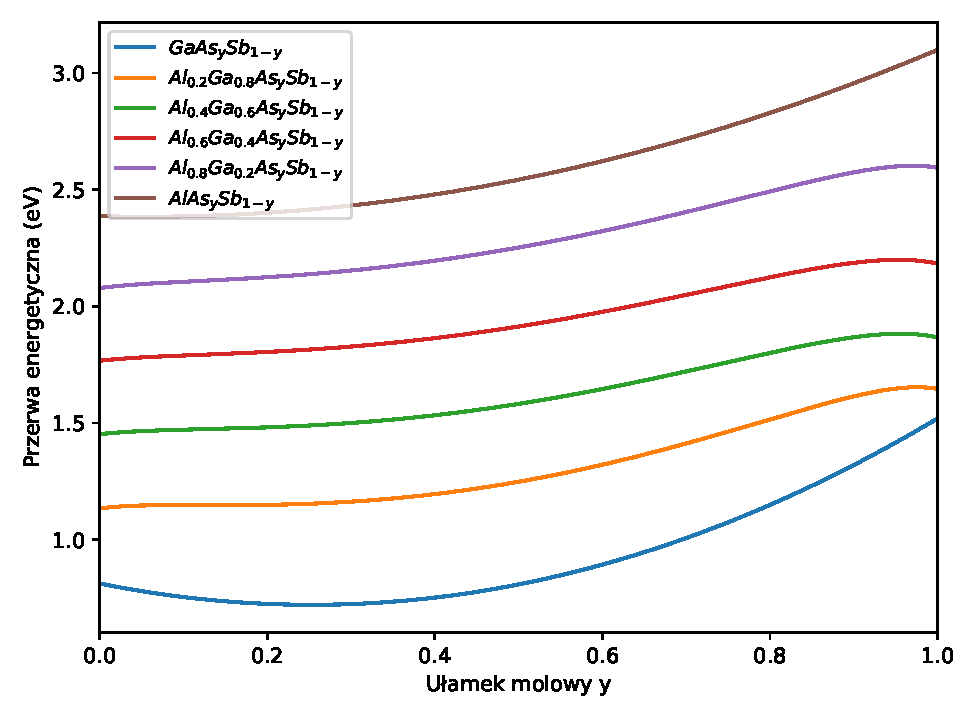
\includegraphics[width = \linewidth]{Figures/quaternary/quat_eg_x.pdf}\label{fig:quat_Eg_x}
\end{minipage}
\begin{minipage}[t]{0.5\textwidth}
	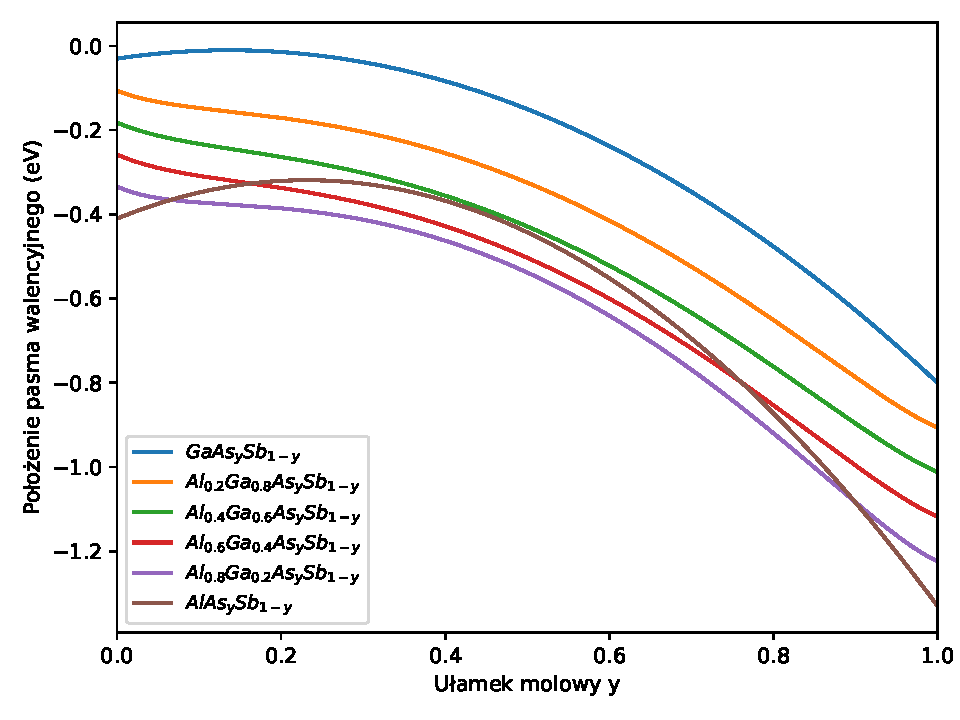
\includegraphics[width = \linewidth]{Figures/quaternary/quat_vbo_x.pdf}\label{fig:quat_vbo_x}
\end{minipage}

\begin{minipage}[t]{0.5\textwidth}
	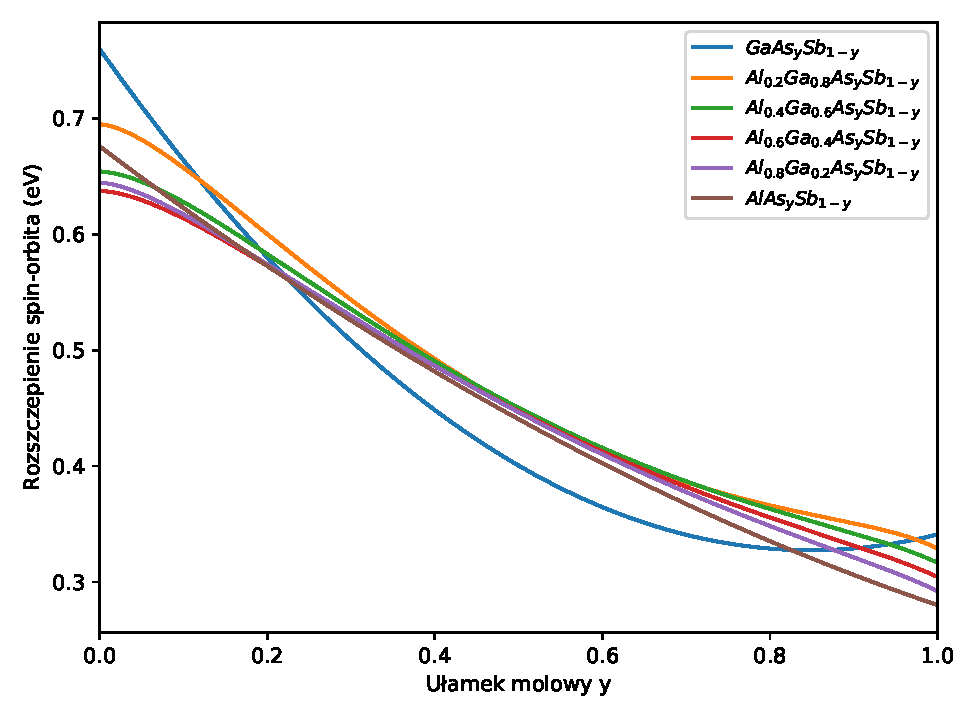
\includegraphics[width = \linewidth]{Figures/quaternary/quat_delta_so_x.pdf}\label{fig:quat_delta_so_x}
\end{minipage}
\begin{minipage}[t]{0.5\textwidth}
	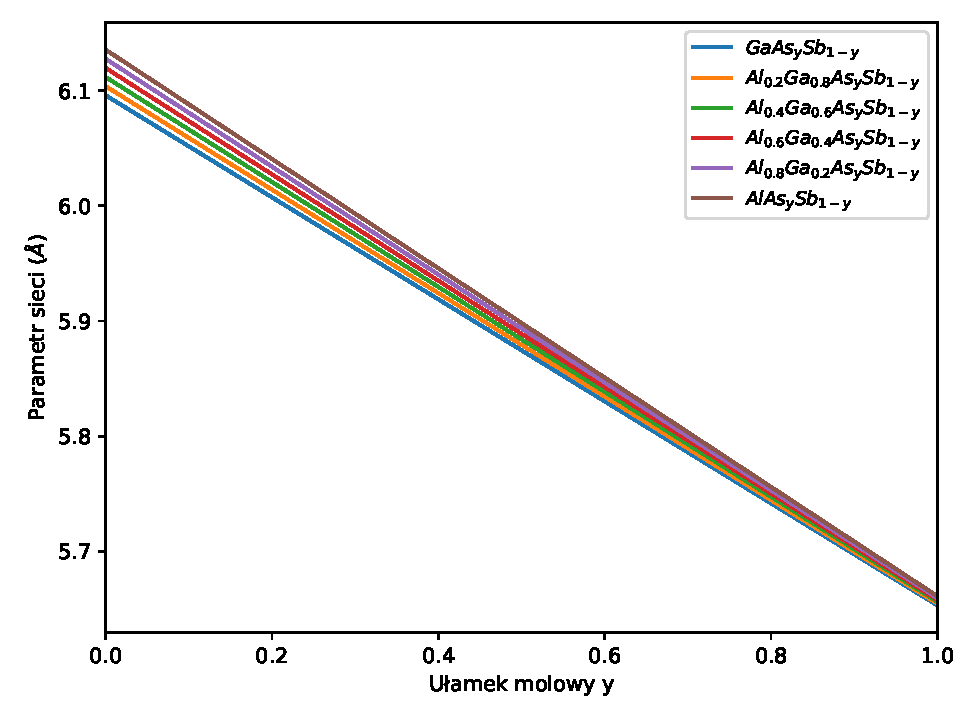
\includegraphics[width = \linewidth]{Figures/quaternary/quat_alc_x.pdf}\label{fig:quat_alc_x}
\end{minipage}

\begin{minipage}[t]{0.5\textwidth}
	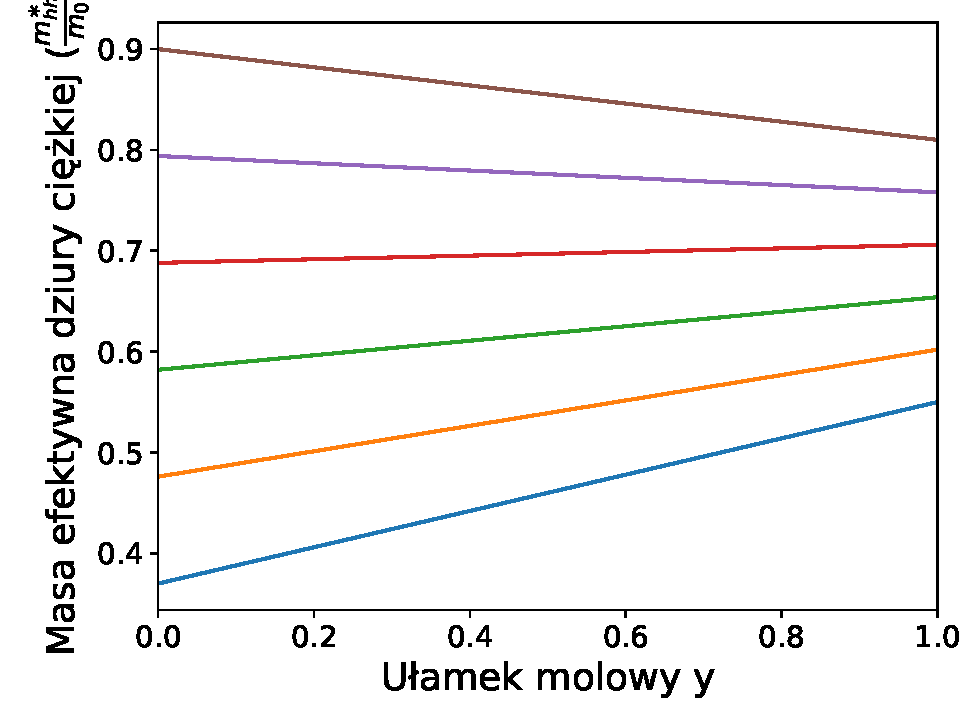
\includegraphics[width = \linewidth]{Figures/quaternary/quat_m_hh_x.pdf}\label{fig:quat_mhh_x}
\end{minipage}
\begin{minipage}[t]{0.5\textwidth}
	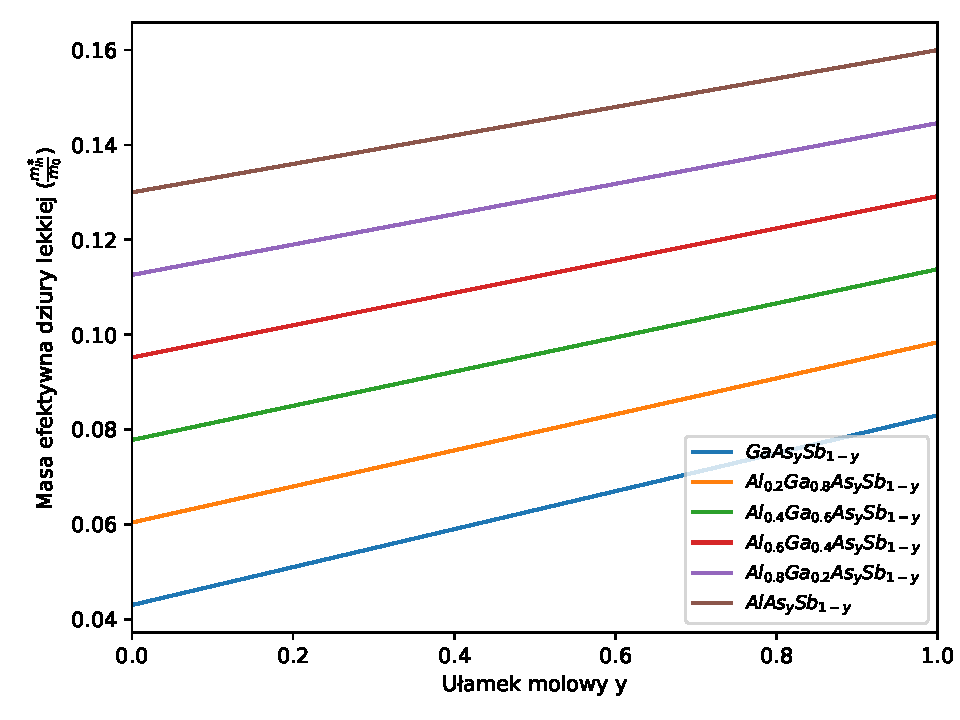
\includegraphics[width = \linewidth]{Figures/quaternary/quat_m_lh_x.pdf}\label{fig:quat_mlh_x}
\end{minipage}

\begin{center}
\begin{minipage}[t]{0.5\textwidth}
	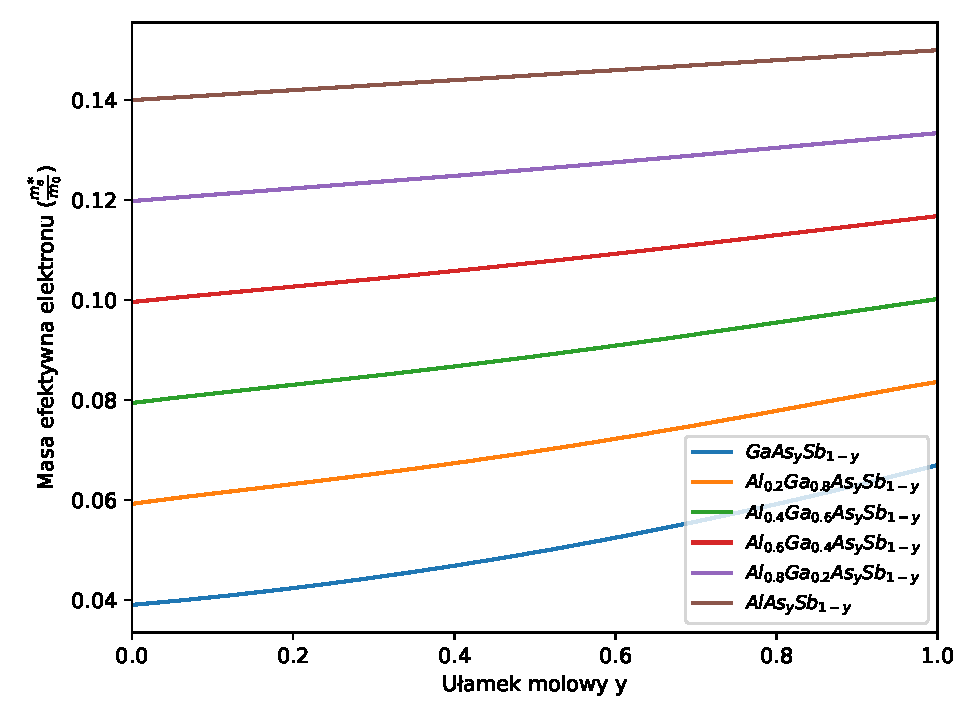
\includegraphics[width = \linewidth]{Figures/quaternary/quat_m_e_x.pdf}\label{fig:quat_me_x}
\end{minipage}
\captionof{figure}{Wykresy parametów stopu czteroskładnikowego dla ustalonego
ułamka molowego \(x\), w funkcji ułamka molowego \(y\).}
\end{center}

\subsection{Ustalony \(y\), zmienny \(x\)}
W drugiej serii wykresów ułamek molowy \(y\) przyjmuje ustalone
wartości wynoszące\\
\([0.0,\;0.2,\; 0.4,\; 0.6,\; 0.8,\; 1.0]\), a ułamek molowy \(x\)
przyjmuje \(1000\) równoodległych wartości między \(0.0\) i \(1.0\). 


\begin{minipage}[t]{0.5\textwidth}
	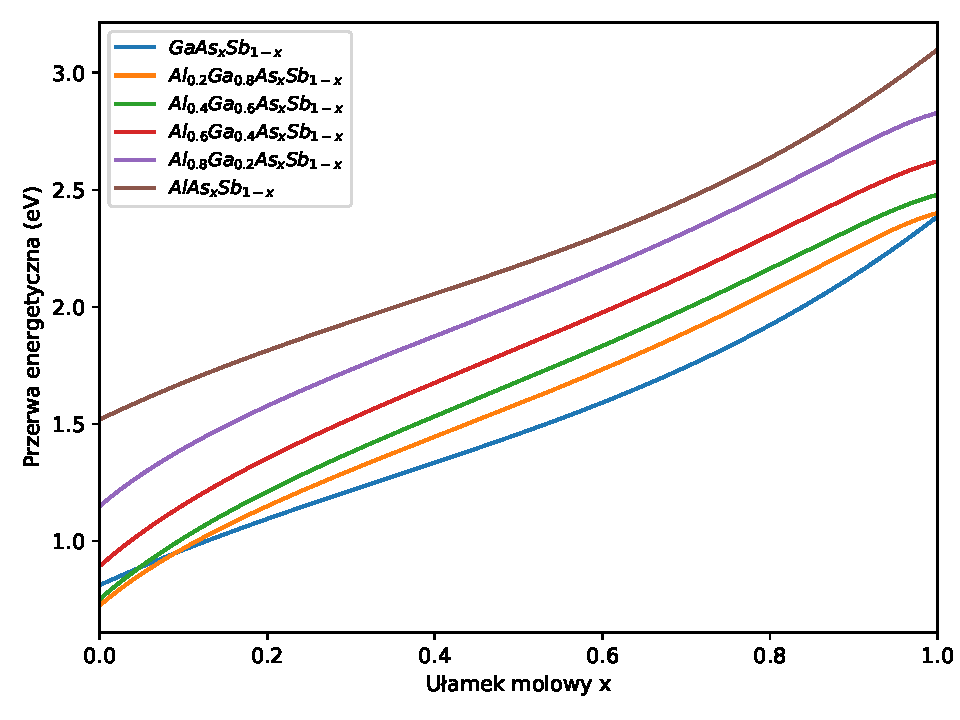
\includegraphics[width = \linewidth]{Figures/quaternary/quat_eg_y.pdf}\label{fig:quat_Eg_y}
\end{minipage}
\begin{minipage}[t]{0.5\textwidth}
	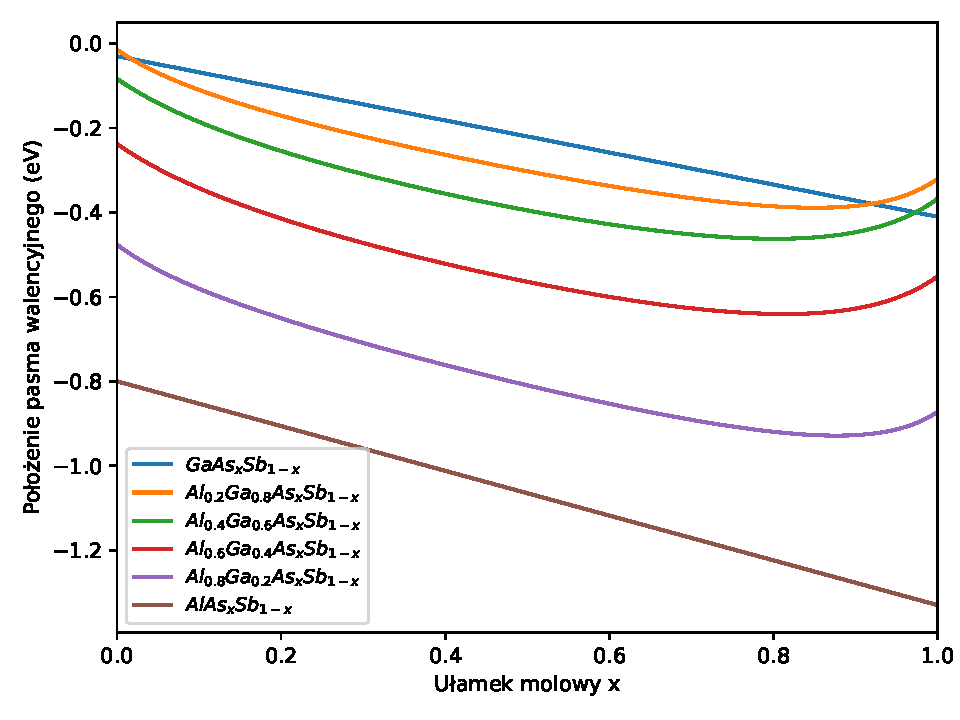
\includegraphics[width = \linewidth]{Figures/quaternary/quat_vbo_y.pdf}\label{fig:quat_vbo_y}
\end{minipage}

\begin{minipage}[t]{0.5\textwidth}
	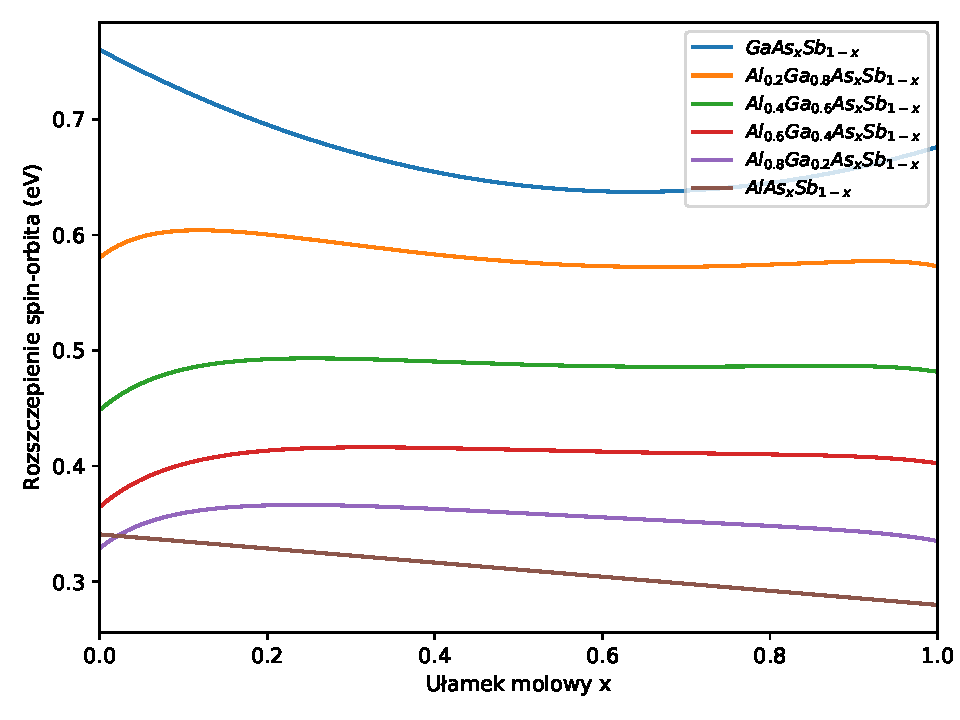
\includegraphics[width = \linewidth]{Figures/quaternary/quat_delta_so_y.pdf}\label{fig:quat_delta_so_y}
\end{minipage}
\begin{minipage}[t]{0.5\textwidth}
	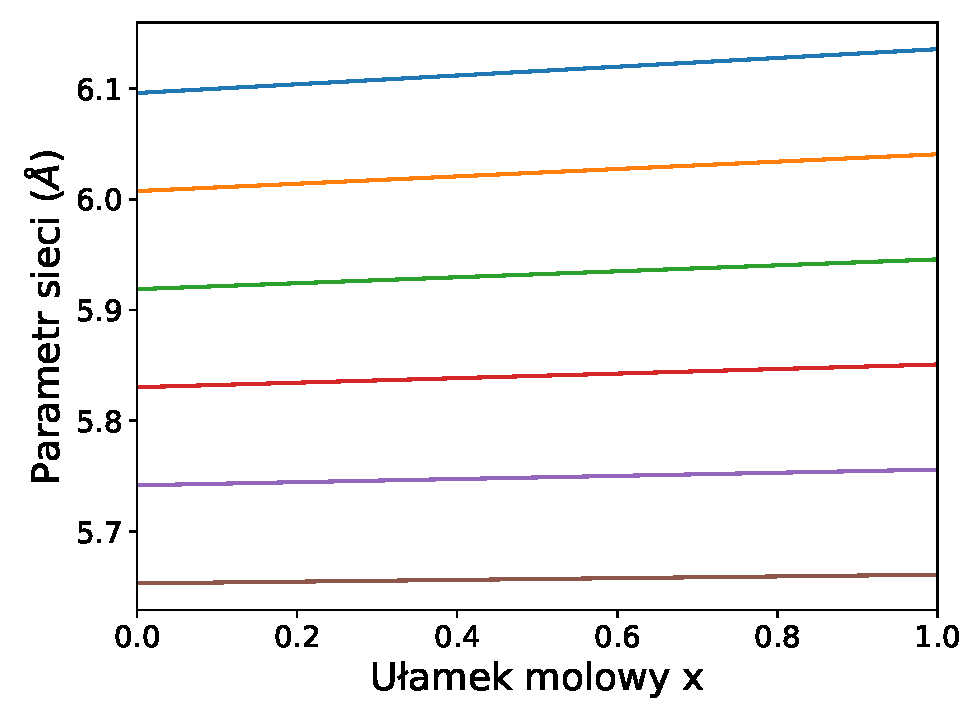
\includegraphics[width = \linewidth]{Figures/quaternary/quat_alc_y.pdf}\label{fig:quat_alc_y}
\end{minipage}

\begin{minipage}[t]{0.5\textwidth}
	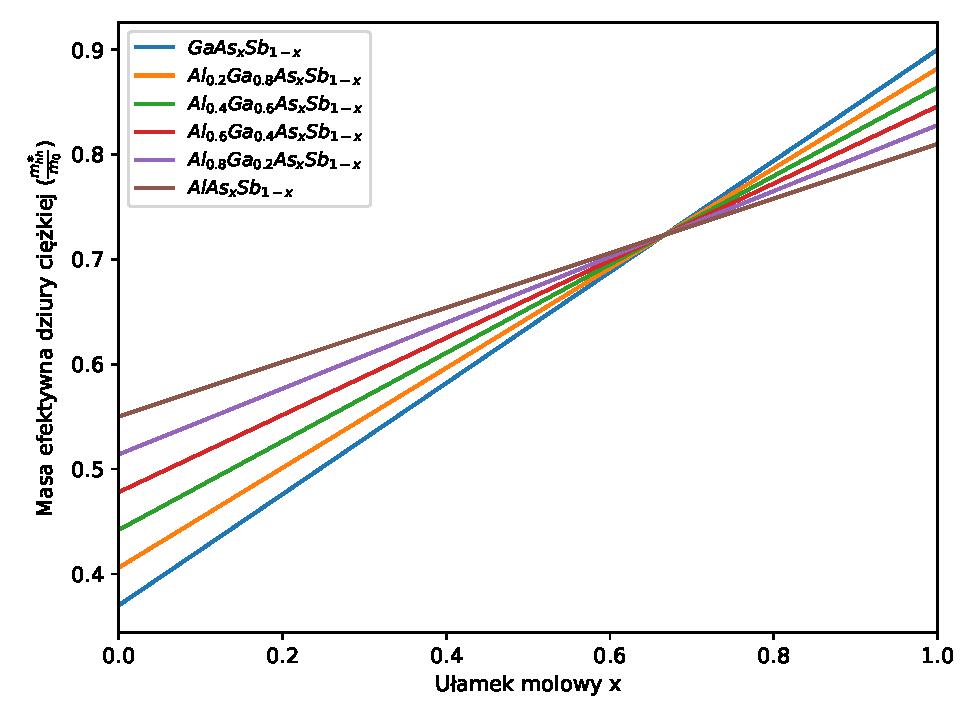
\includegraphics[width = \linewidth]{Figures/quaternary/quat_m_hh_y.pdf}\label{fig:quat_mhh_y}
\end{minipage}
\begin{minipage}[t]{0.5\textwidth}
	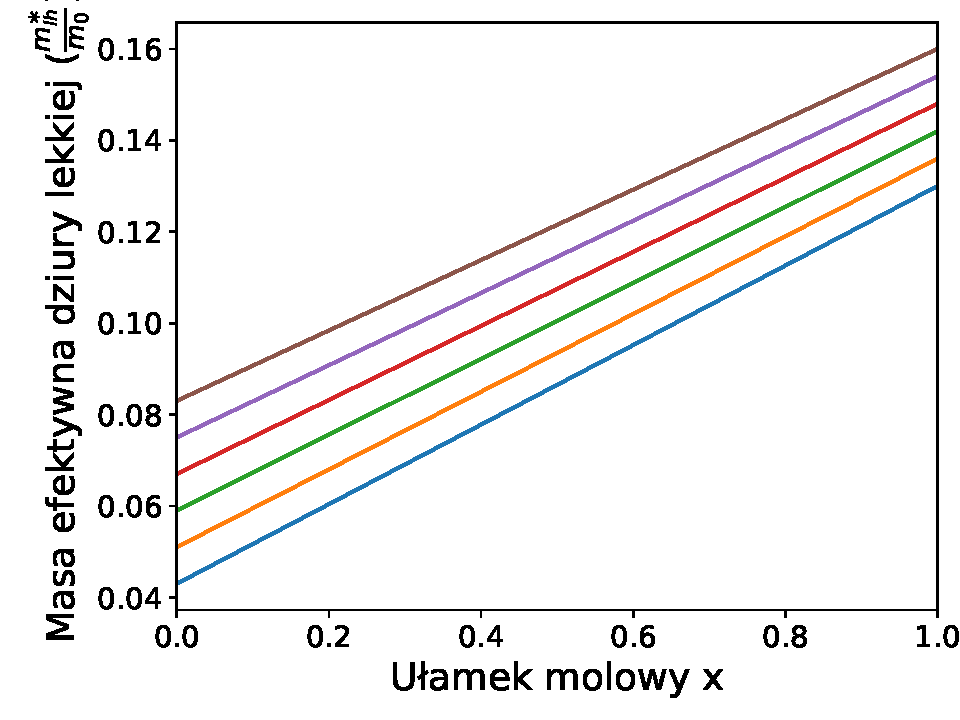
\includegraphics[width = \linewidth]{Figures/quaternary/quat_m_lh_y.pdf}\label{fig:quat_mlh_y}
\end{minipage}

\begin{center}
\begin{minipage}[t]{0.5\textwidth}
	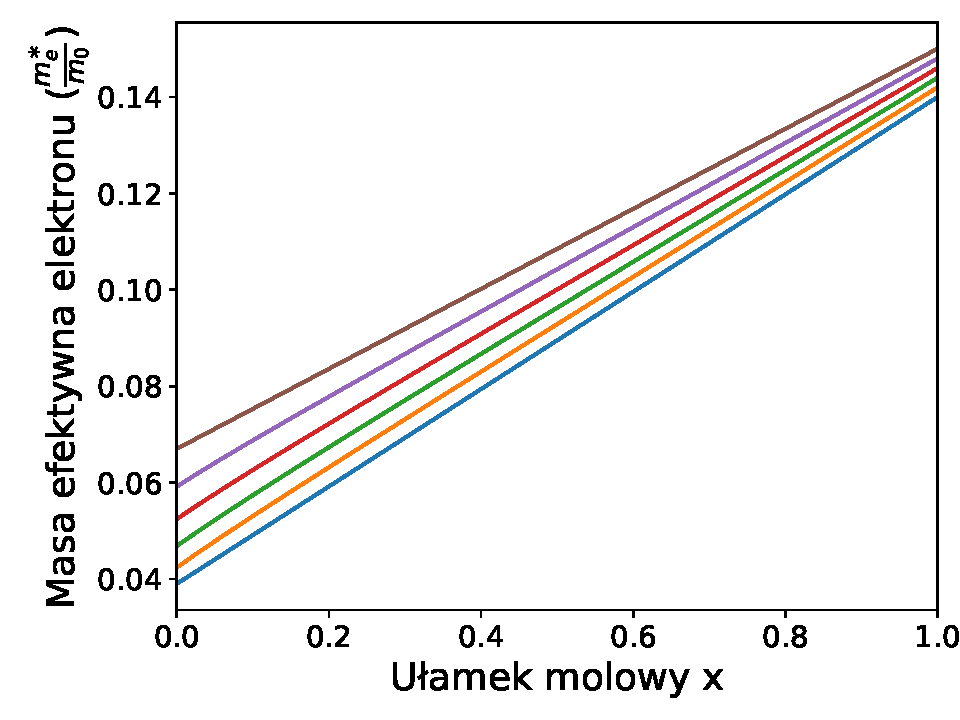
\includegraphics[width = \linewidth]{Figures/quaternary/quat_m_e_y.pdf}\label{fig:quat_me_y}
\end{minipage}
\captionof{figure}{Wykresy parametów stopu czteroskładnikowego dla ustalonego
ułamka molowego \(y\), w funkcji ułamka molowego \(x\).}
\end{center}


\section{Odkształcenia przy wzroście epitaksjalnym na podłożu GaAs. Wpływ temperatury.}\label{sec:strain}

W tej sekcji przeanalizujemy wpływ naprężeń na energie pasm w \BPChem{AlGaAsSb}. odkształcenia zostaną wprowadzone
jako konsekwencja wzrostu epitaksjalnego na podłożu \BPChem{GaAs}. 

\begin{table}[htbp]
	\centering
\caption{Parametry Varshiego materiałów binarnych. Zależności parametru sieci od temperatury.}
\begin{tabular}{ccccc}
	\toprule
	\toprule
	Parametr & \BPChem{AlAs} & \BPChem{AlSb} &  \BPChem{GaSb} & \BPChem{GaAs}\\
	\midrule
	\(\alpha\) (meV/K)  	& 0.885 & 0.42 & 0.417 & 0.5405  \\
	\(\beta\) (K)   		& 530   & 140  & 140   & 204     \\
	\(a_{lc}^T\) (\AA/K)  	& 2.9   & 2.6  & 4.72  & 3.88    \\
	\bottomrule
  \bottomrule  
  \end{tabular}%
	\label{tab:temp}%
  \end{table}%

\begin{figure}[H]
	\centering
	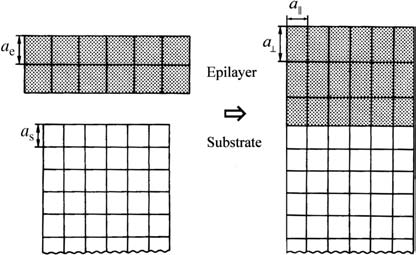
\includegraphics[width = 0.7\textwidth]{Figures/strain.jpg}
	\caption{Przekrój poprzeczny przez próbkę. Parametry sieciowe warstwy wzrostowej oraz podłoża oznaczone są odpowiednio
	\(a_e\) oraz \(a_s\). Źródło:~\citetitle{Adachi2009},~\textcite{Adachi2009}.}\label{fig:strain}
\end{figure}

W pierwszej kolejności uwzględniony zostanie wpływ temperatury na szerokość w przerwy wzbronionej
oraz parametru sieci materiałów binarnych. Zależność temperaturowa przerwy wzbronionej opisana jest
przy pomocy parametrów Varshiego \(\alpha\) i \(\beta\) oraz równania~\autocite{Vurgaftman2001}:
\begin{equation}
	E_g(T) = E_g(T=0) - \frac{\alpha \cdot T^2}{T + \beta}\label{eq:varshi}
\end{equation}
Zależność temperaturowa parametru sieci dana jest równaniem:
\begin{equation}
	a_{lc}(T) = a_{lc}(T = 0) + a_{lc}^T \cdot 10^{-5}\cdot(T - 300)
\end{equation}
Parametry Varshiego materiałów binarnych, oraz zależności parametru sieci od temperatury przedstawione są w tabeli~\ref{tab:temp}:


W celu wyznaczenia temperaturowej zależności parametrów dla stopów trójskładnikowych i czteroskładnikowego,
posłużono się schematem interpolacyjnym opisanym w~\ref{sec:interpolation}.
  

\begin{table}[htbp]
	\centering
\caption{Potencjały deformacyjne oraz parametry sztywności materiałów binarnych~\autocite{Vurgaftman2001}.}
\begin{tabular}{ccccc}
	\toprule
	\toprule
	Parametr & \BPChem{AlAs} & \BPChem{AlSb} &  \BPChem{GaSb} & \BPChem{GaAs}\\
	\midrule
	\(a_{c}\)   (eV)  	& -5.64 & -4.5   & -7.5   & -7.17 \\
	\(a_{v}\)   (eV)   	& -2.47 & -1.4   & -0.8   & -1.16 \\
	\(b\)      (eV)  	& -2.3  & -1.35  & -2.0   & -2.0  \\
	\(C_{11}\) (GPa)  	&  1250 &  876.9 &  884.2 &  1221 \\
	\(C_{12}\) (GPa)  	&  534  &  434.1 &  402.6 &  566  \\
\bottomrule
  \bottomrule  
  \end{tabular}%
	\label{tab:strain_params}%
  \end{table}%

\begin{minipage}[t]{0.5\textwidth}
	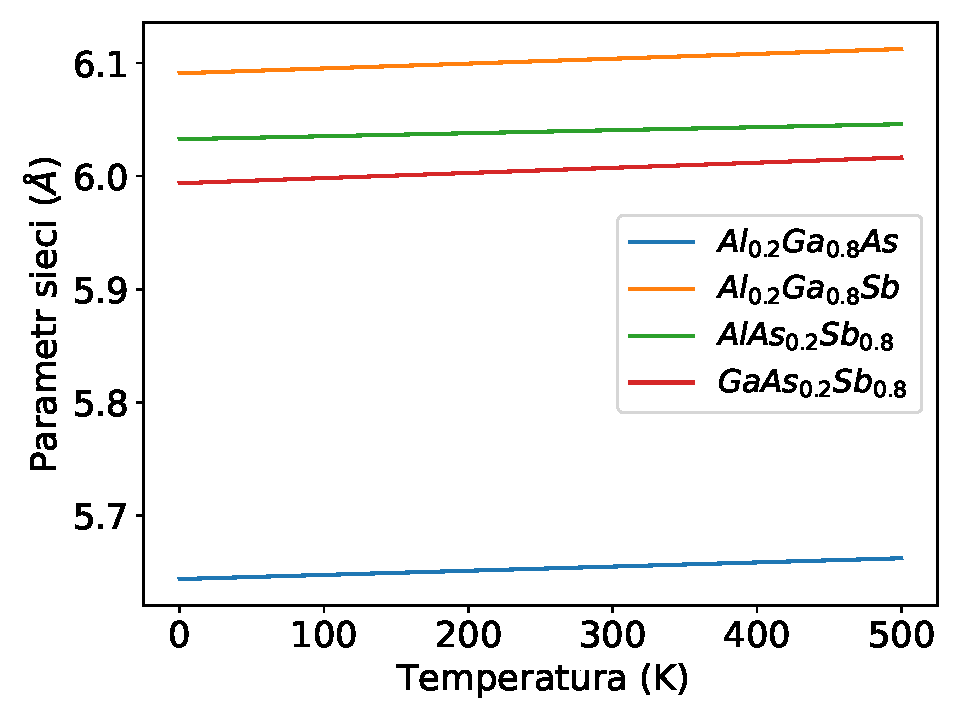
\includegraphics[width = \linewidth]{Figures/strain/ter_alc1.pdf}\label{fig:ter_alc1}
\end{minipage}
\begin{minipage}[t]{0.5\textwidth}
	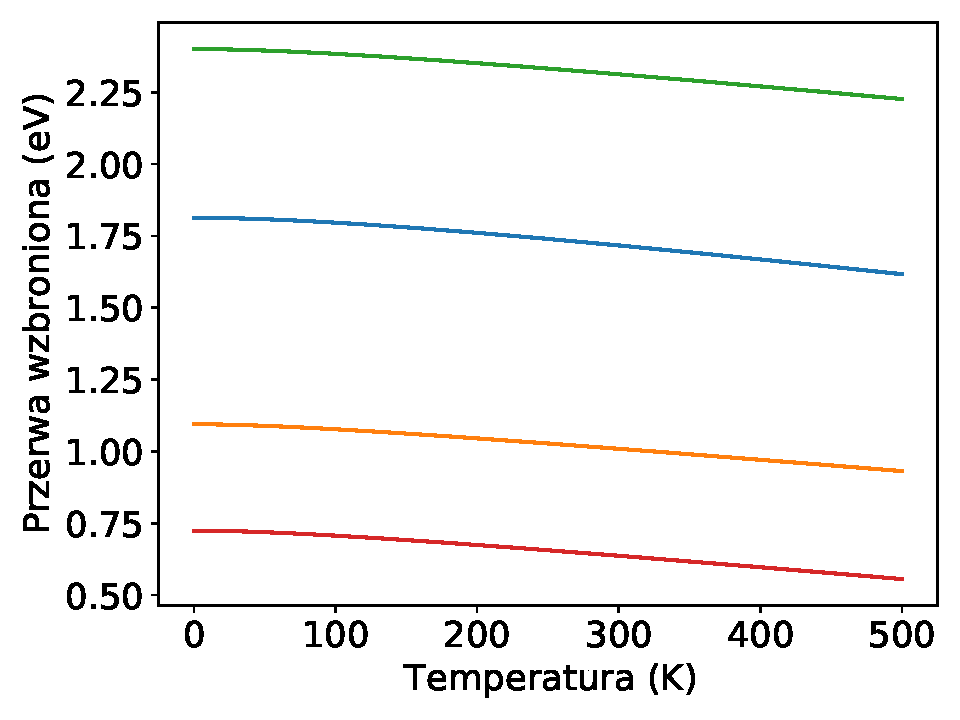
\includegraphics[width = \linewidth]{Figures/strain/ter_eg1.pdf}\label{fig:ter_eg1}
\end{minipage}

\begin{minipage}[t]{0.5\textwidth}
	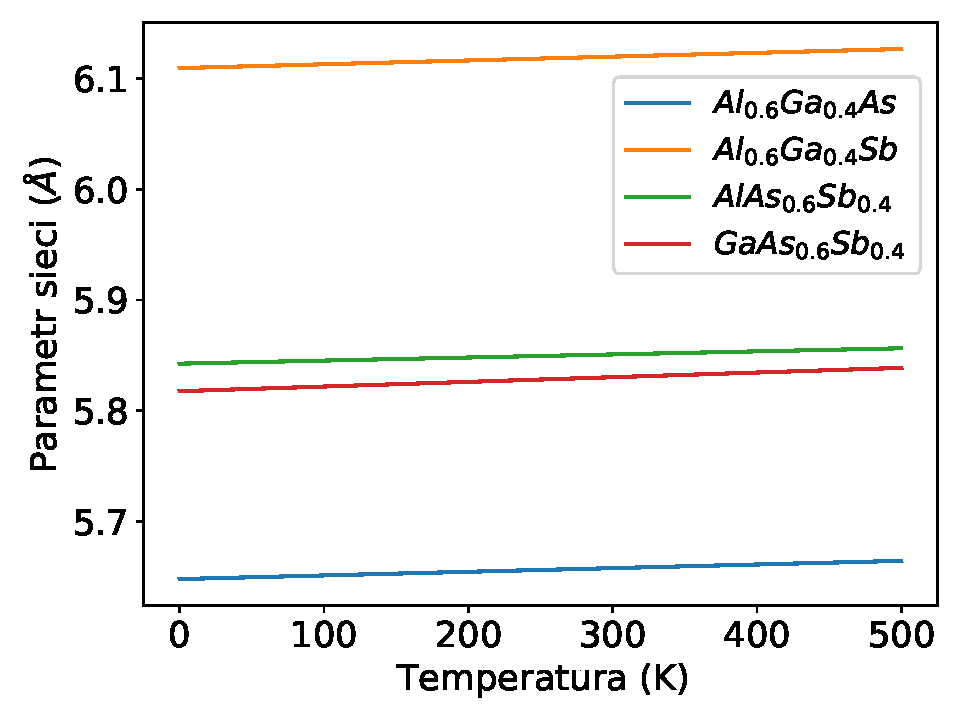
\includegraphics[width = \linewidth]{Figures/strain/ter_alc2.pdf}\label{fig:ter_alc1}
\end{minipage}
\begin{minipage}[t]{0.5\textwidth}
	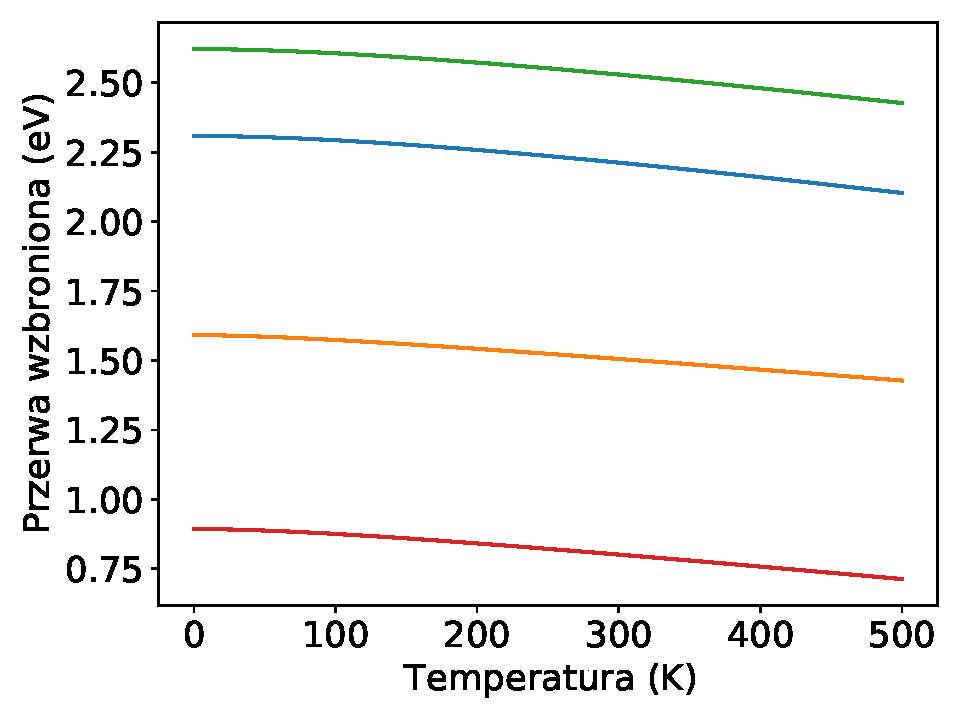
\includegraphics[width = \linewidth]{Figures/strain/ter_eg2.pdf}\label{fig:ter_eg2}
\end{minipage}
\begin{center}
\captionof{figure}{Zależności interpolowanej przerwy wzbronionej i parametru sieci dla stopów 
trójskładnikowych, i wybranych ułamków molowych \(x\).}
\end{center}

Znając zależność temperaturową stopu czteroskładnikowego oraz podłoża policzono
odkształcenia występujące w próbce. Potrzebne potencjały deformacyjne oraz parametry sztywności
zostały wyznaczone przy pomocy standardowego schematu interpolacyjnego dla stopu czteroskładnikowego.
Ze względu na brak dostępności parametrów nieliniowości ograniczono się do interpolacji liniowej.

  
Do obliczenia wpływu naprężeń posłużono się następującymi wzorami:
\begin{align}
	\label{eq:strains}
	&\varepsilon_{\parallel } \equiv \varepsilon_{xx} = \varepsilon_{yy} = \frac{a_{GaAs} - a_{AlGaAsSb}}{a_{AlGaAsSb}}\\ \nonumber
	&\varepsilon_{\perp } \equiv \varepsilon_{zz} = -2\frac{C_{12}}{C_{11}}\varepsilon_{\parallel}\\ \nonumber
	&\delta E_{c,hydro} = a_c\left(\varepsilon_{\perp} + 2\varepsilon_{\parallel}\right)\\ \nonumber
	&\delta E_{v,hydro} = a_v\left(\varepsilon_{\perp} + 2\varepsilon_{\parallel}\right)\\ \nonumber
	&\delta E_{v,biax} = b\left(\varepsilon_{\perp} - \varepsilon_{\parallel}\right)\\ \nonumber
	&\delta E_{v,biax}^{\pm} = \frac{1}{2}\left(\delta E_{v,biax} - \Delta_{SO} \pm \sqrt{9\delta E_{v,biax}^2 + 2\delta E_{v,biax} \Delta_{SO} + \Delta_{SO}^2 }\right)\\ \nonumber
\end{align}
W przypadku braku indeksu górnego lub dolnego, przyjmujemy że stałe są obliczone
dla stopu czteroskładnikowego. Przyjmujemy, że nasz materiał ma wzór stechiometryczny
\BPChem{Al\_{x}Ga\_{1-x}As\_{y}Sb\_{1-y}}.

\begin{minipage}[t]{0.5\textwidth}
	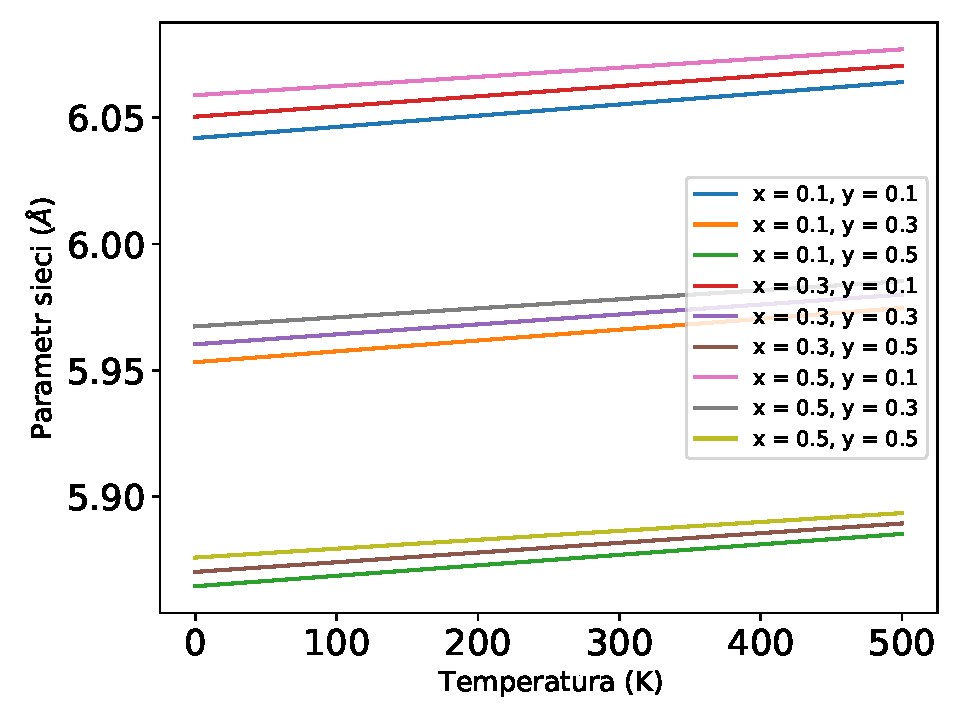
\includegraphics[width = 0.9\linewidth]{Figures/strain/alc1.pdf}\label{fig:alc1}
\end{minipage}
\begin{minipage}[t]{0.5\textwidth}
	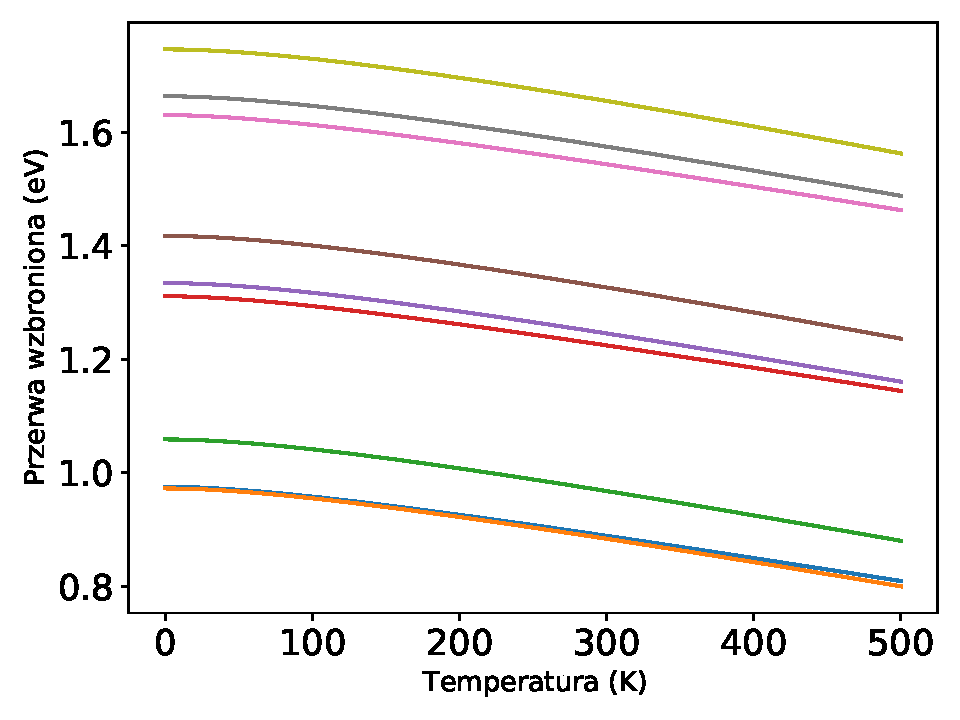
\includegraphics[width = 0.9\linewidth]{Figures/strain/eg1.pdf}\label{fig:eg1}
\end{minipage}

\begin{minipage}[t]{0.5\textwidth}
	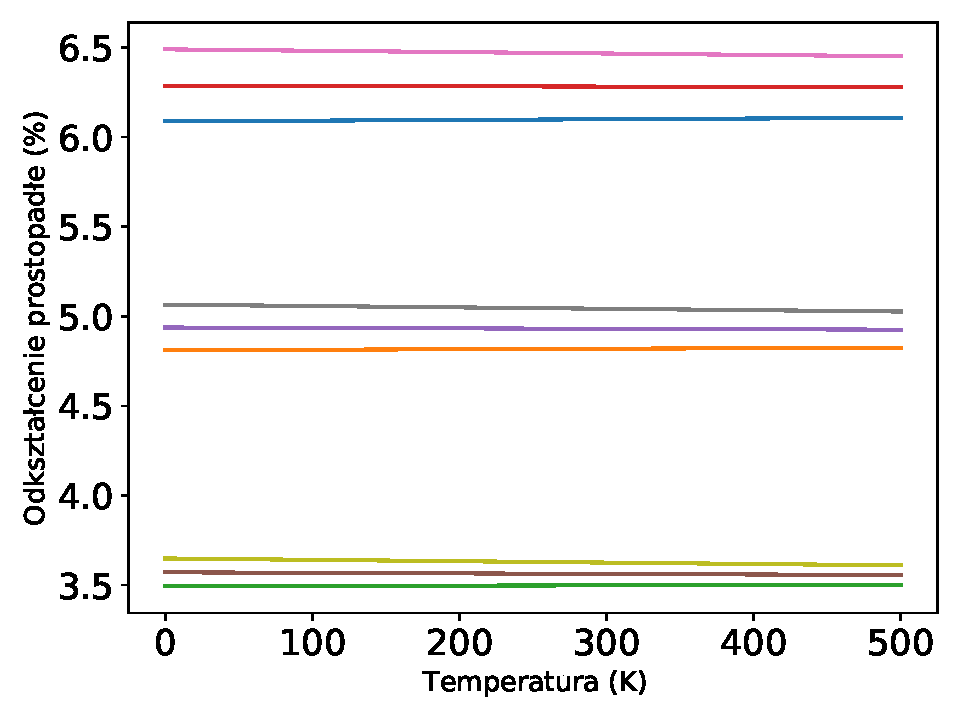
\includegraphics[width = 0.9\linewidth]{Figures/strain/eps_orth1.pdf}\label{fig:eps_orth1}
\end{minipage}
\begin{minipage}[t]{0.5\textwidth}
	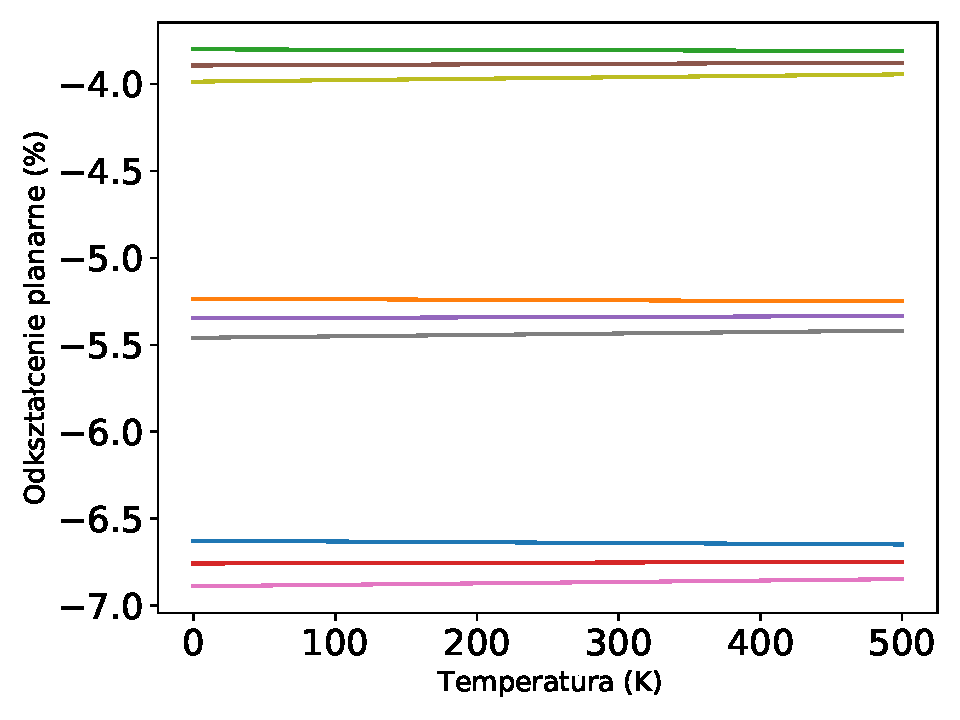
\includegraphics[width = 0.9\linewidth]{Figures/strain/eps_par1.pdf}\label{fig:eps_par1}
\end{minipage}
\begin{center}
\captionof{figure}{Zależności interpolowanej przerwy wzbronionej i parametru sieci dla stopu czteroskładnikowego
od temperatury. Odkształcenia prostopadłe oraz planarne w funkcji temperatury.}\label{fig:grp1}
\end{center}

\begin{minipage}[t]{0.5\textwidth}
	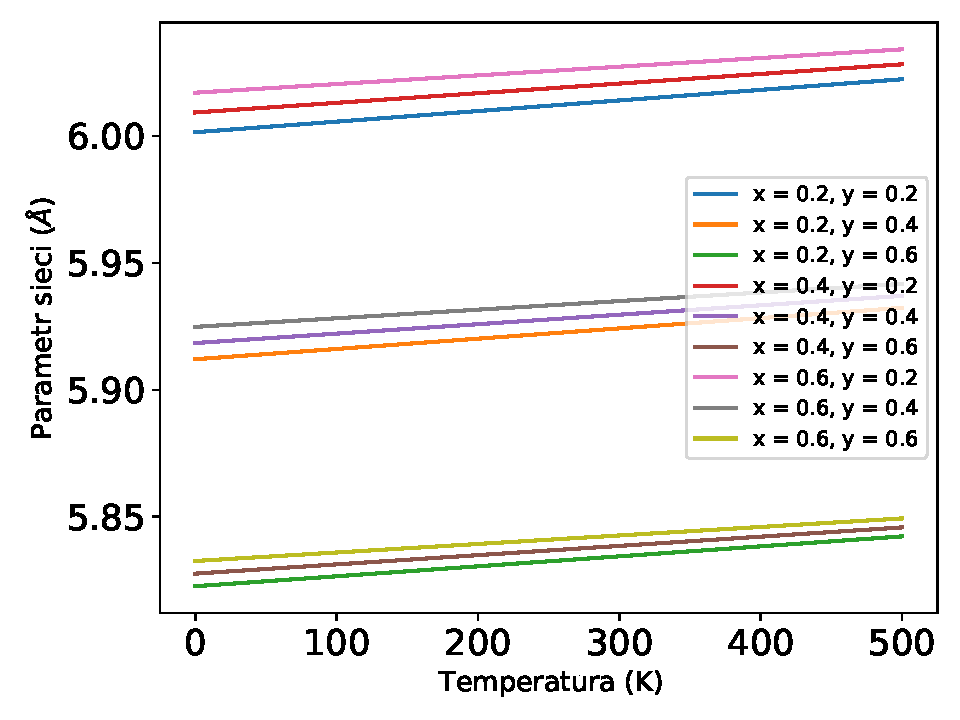
\includegraphics[width = 0.9\linewidth]{Figures/strain/alc2.pdf}\label{fig:alc2}
\end{minipage}
\begin{minipage}[t]{0.5\textwidth}
	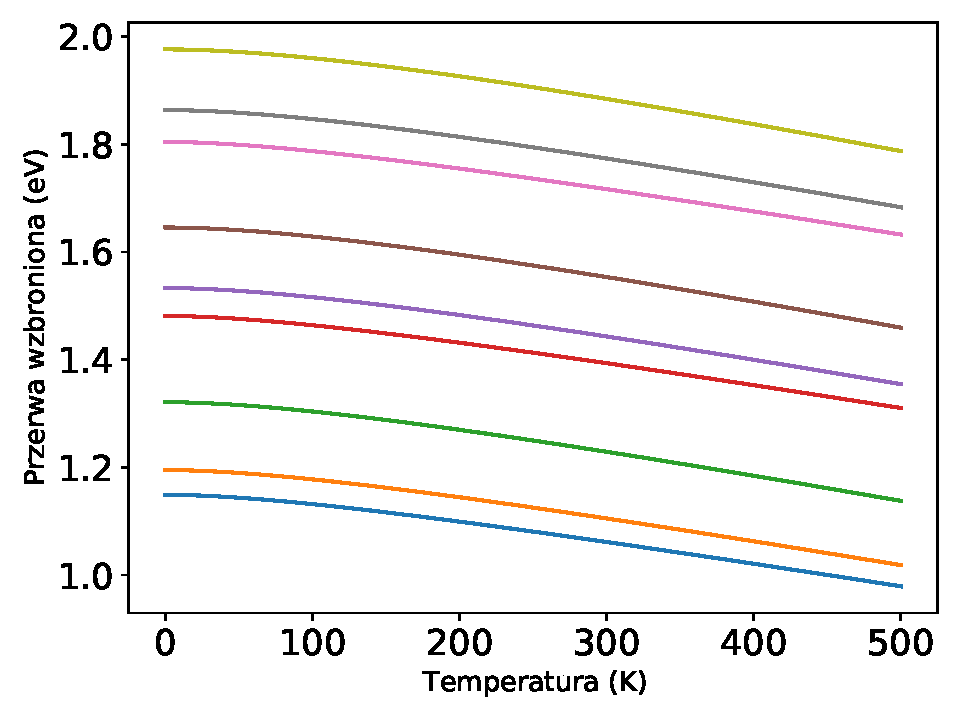
\includegraphics[width = 0.9\linewidth]{Figures/strain/eg2.pdf}\label{fig:eg2}
\end{minipage}

\begin{minipage}[t]{0.5\textwidth}
	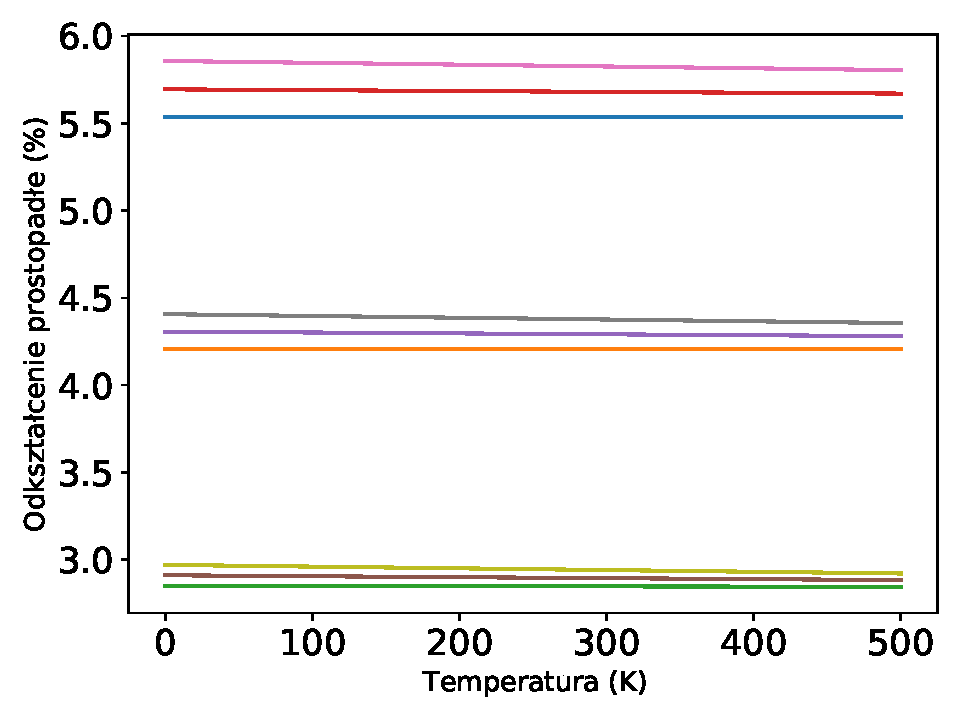
\includegraphics[width = 0.9\linewidth]{Figures/strain/eps_orth2.pdf}\label{fig:eps_orth2}
\end{minipage}
\begin{minipage}[t]{0.5\textwidth}
	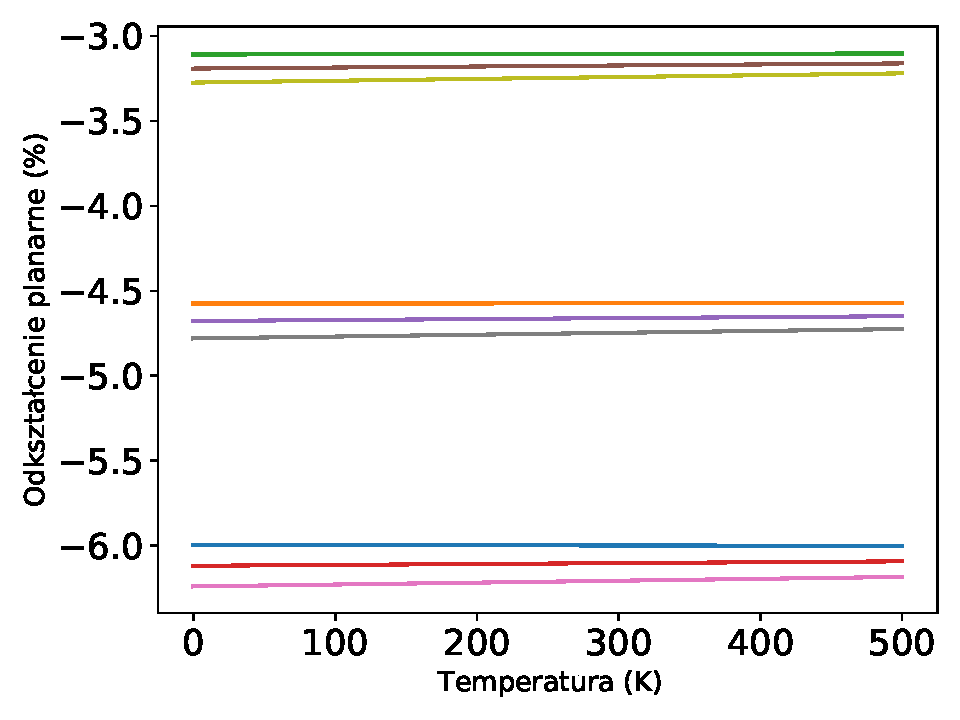
\includegraphics[width = 0.9\linewidth]{Figures/strain/eps_par2.pdf}\label{fig:eps_par2}
\end{minipage}
\begin{center}
\captionof{figure}{To samo co na rysunku~\ref{fig:grp1}, ale dla innych ustalonych ułamków molowych \(x\) i \(y\).}
\end{center}

Powyższe obliczenia pozwoliły na uzyskanie energii pasm w funkcji temperatury, z uwzględnieniem jej
wpływu na Odkształcenia. Policzono odpowiednio: energię pasma przewodnictwa, energię pasma walencyjnego
dziur ciężkich, energię pasma walencyjnego dziur lekkich oraz energię pasma walencyjnego rozszczepionego
poprzez oddziaływanie spin-orbitalne. Wszystkie energie liczone są w punkcie \(\Gamma\)
strefy Brillouina, czyli w poniższych sumach nie pojawia się wkład związany z energią kinetyczną.

\begin{align*}
	E_c &= \textrm{VBO} + E_g + \delta E_{c,hydro}\\
	E_{v,hh} &= \textrm{VBO} + \delta E_{v,hydro} - \delta E_{v,biax}\\
	E_{v,lh} &= \textrm{VBO} + \delta E_{v,hydro} + \delta E_{v,biax}^{+}\\
	E_{v,sh} &= \textrm{VBO} + \delta E_{v,hydro} + \delta E_{v,biax}^{-}\\
\end{align*}

Poniżej przedstawiono rezultaty obliczeń w funkcji temperatury, dla wybranych wartości ułamków molowych \(x\) oraz \(y\).

\begin{minipage}[t]{0.5\textwidth}
	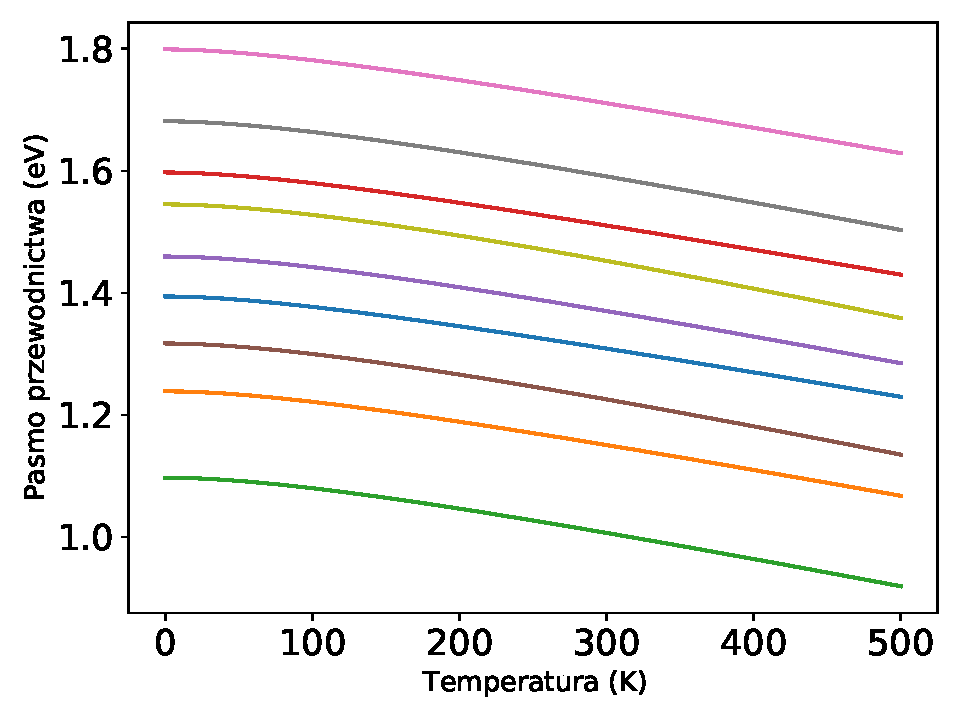
\includegraphics[width = \linewidth]{Figures/strain/Ec1.pdf}\label{fig:Ec1}
\end{minipage}
\begin{minipage}[t]{0.5\textwidth}
	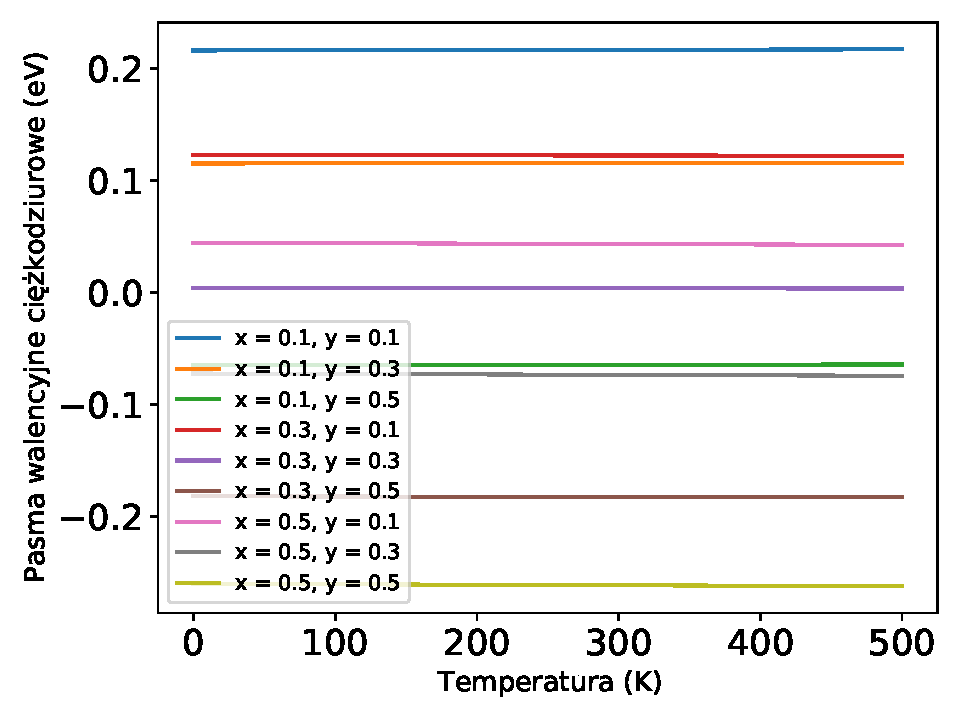
\includegraphics[width = \linewidth]{Figures/strain/Ev_hh1.pdf}\label{fig:Ev_hh1}
\end{minipage}

\begin{minipage}[t]{0.5\textwidth}
	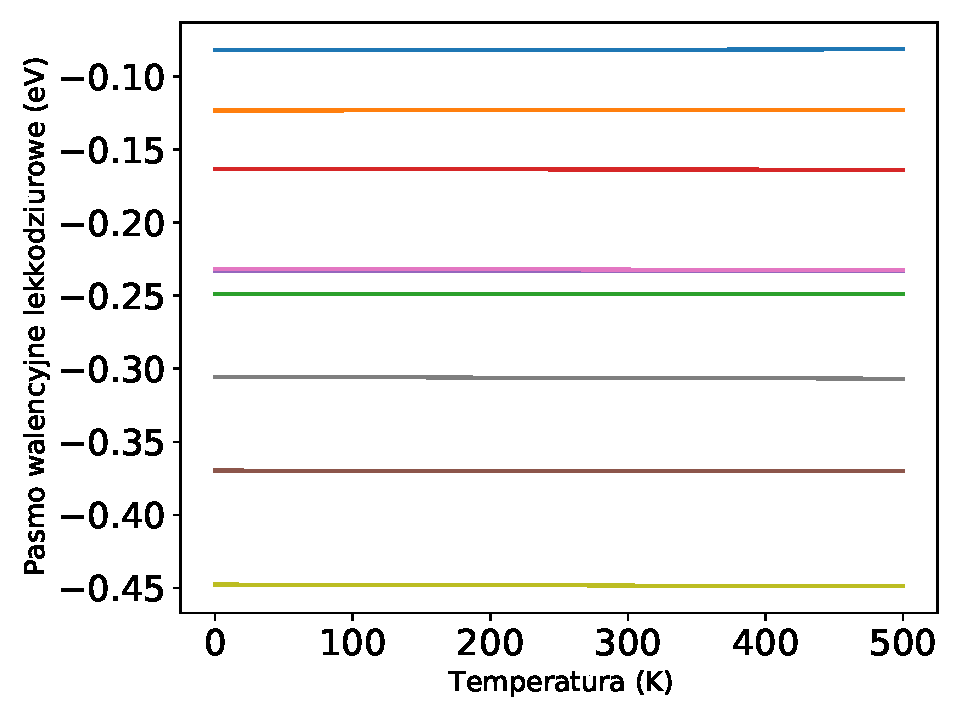
\includegraphics[width = \linewidth]{Figures/strain/Ev_lh1.pdf}\label{fig:Ev_lh1}
\end{minipage}
\begin{minipage}[t]{0.5\textwidth}
	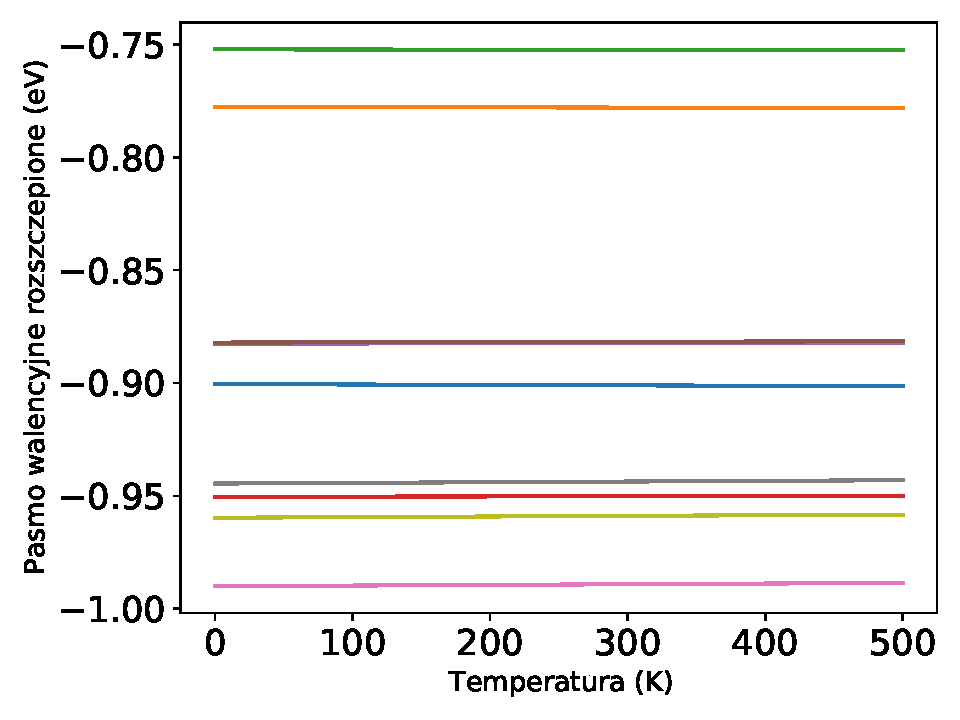
\includegraphics[width = \linewidth]{Figures/strain/Ev_sh1.pdf}\label{fig:Ev_sh1}
\end{minipage}
\begin{center}
\captionof{figure}{Zależności energii czterech badanych pasm od temperatury.}\label{fig:bands1}
\end{center}

\begin{minipage}[t]{0.5\textwidth}
	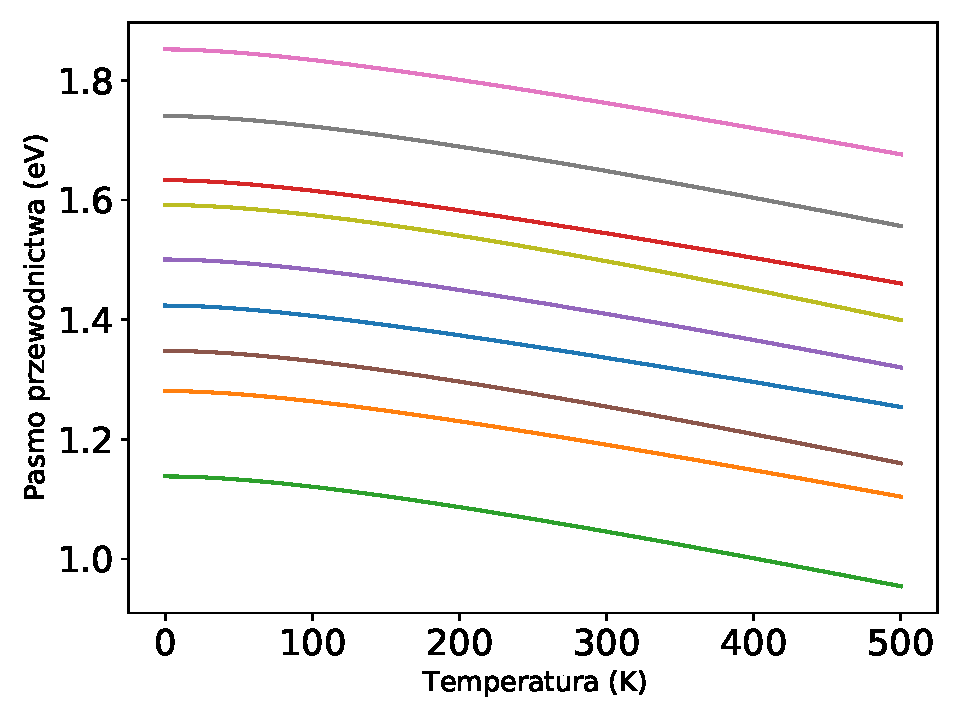
\includegraphics[width = \linewidth]{Figures/strain/Ec2.pdf}\label{fig:Ec2}
\end{minipage}
\begin{minipage}[t]{0.5\textwidth}
	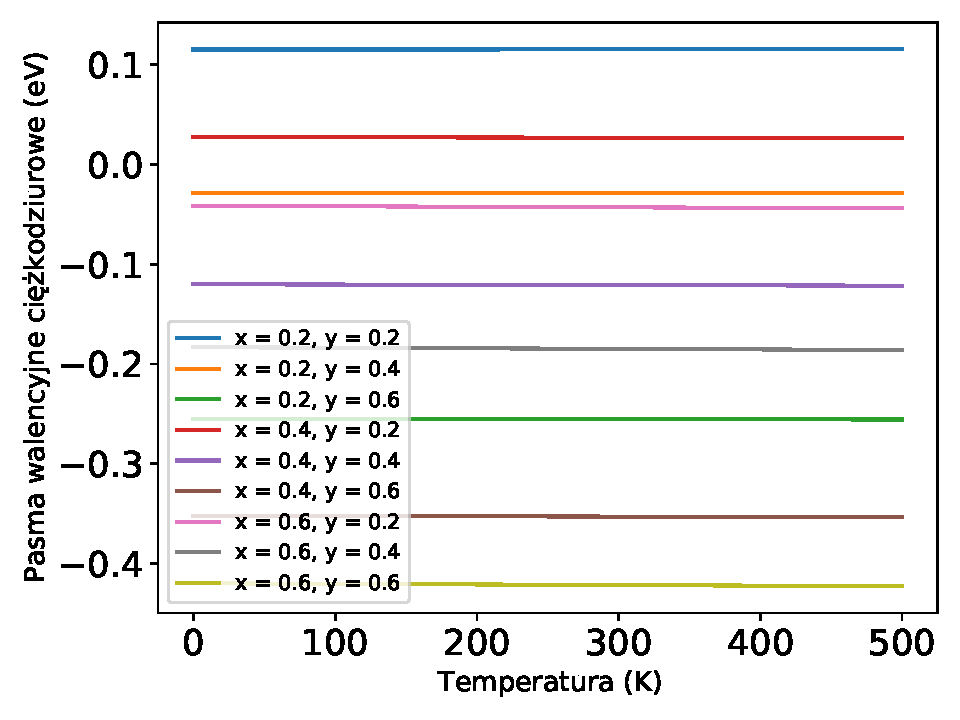
\includegraphics[width = \linewidth]{Figures/strain/Ev_hh2.pdf}\label{fig:Ev_hh2}
\end{minipage}

\begin{minipage}[t]{0.5\textwidth}
	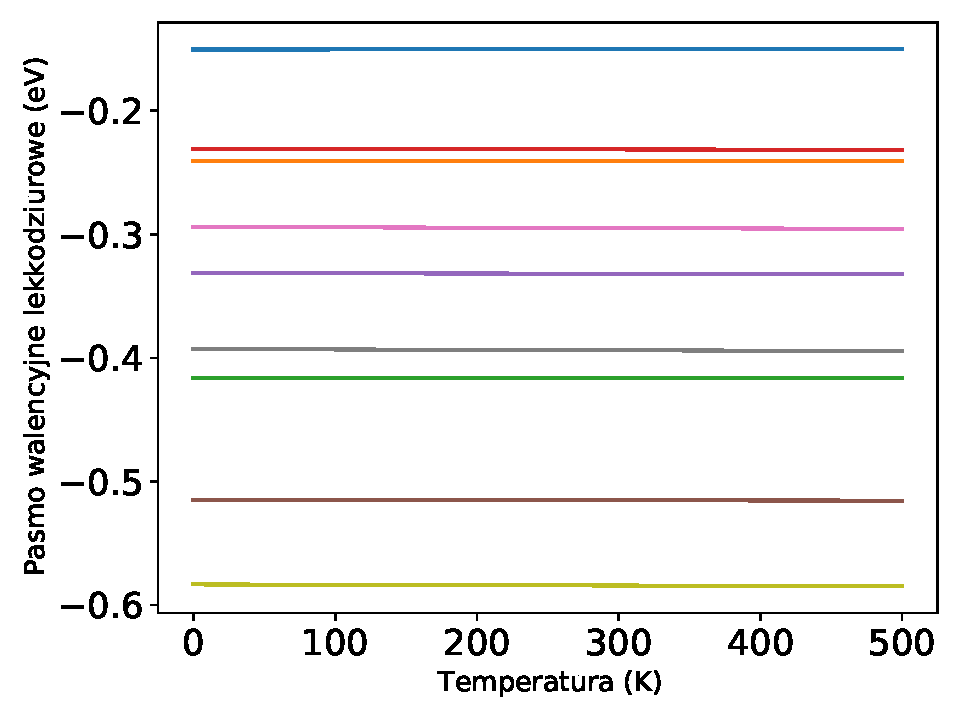
\includegraphics[width = \linewidth]{Figures/strain/Ev_lh2.pdf}\label{fig:Ev_lh2}
\end{minipage}
\begin{minipage}[t]{0.5\textwidth}
	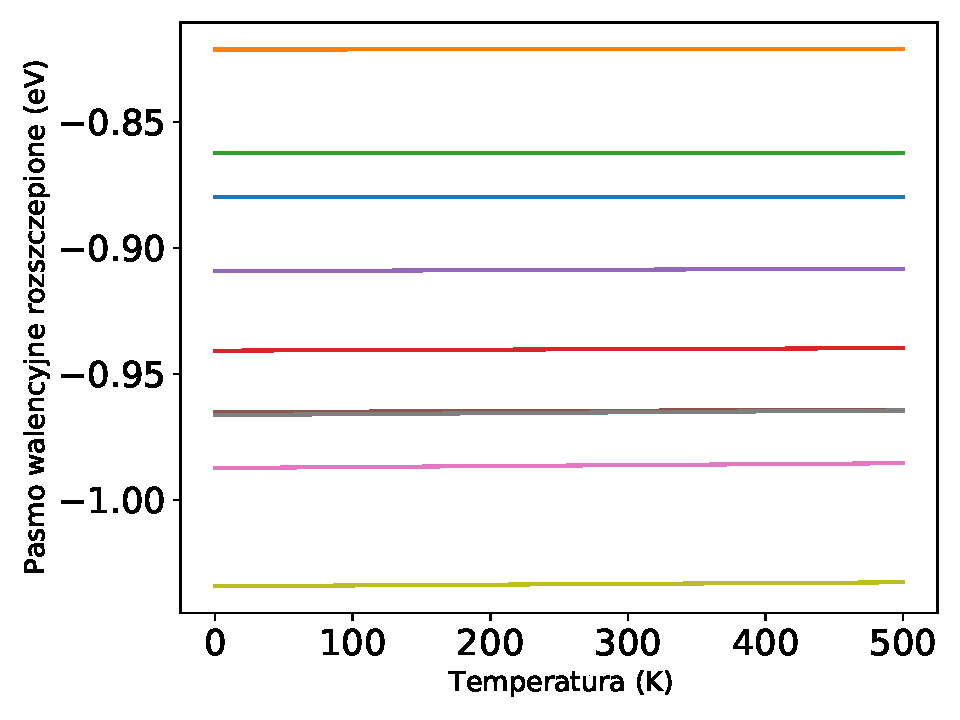
\includegraphics[width = \linewidth]{Figures/strain/Ev_sh2.pdf}\label{fig:Ev_sh2}
\end{minipage}
\begin{center}
\captionof{figure}{To samo co rysunek~\ref{fig:bands1}, tylko dla innych wartości ułamków molowych.}\label{fig:bands2}
\end{center}


\begin{figure}[H]
	\centering
	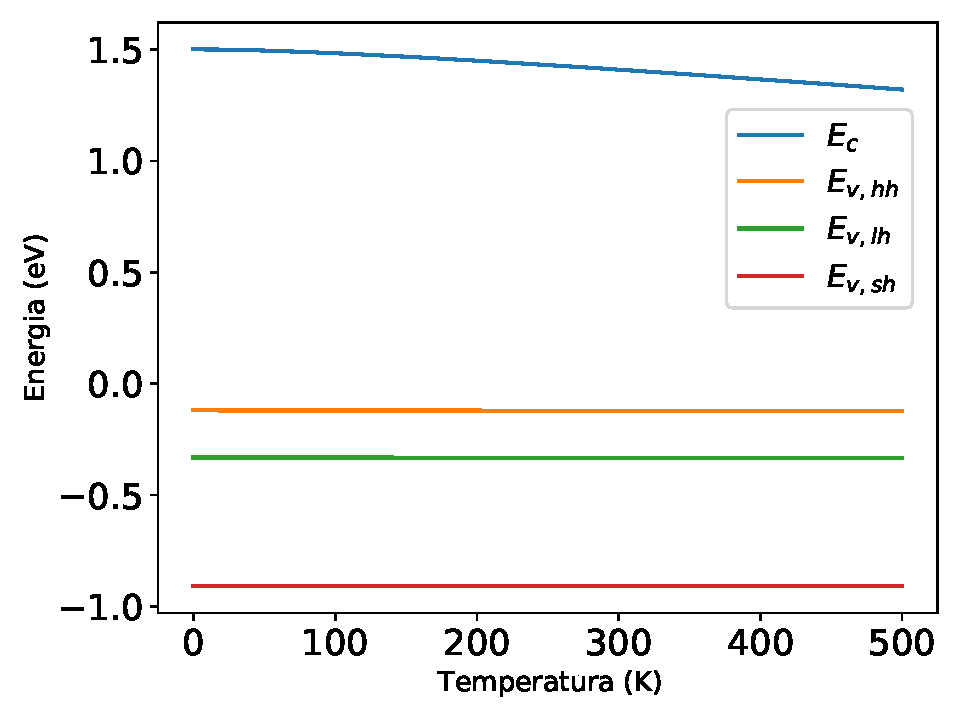
\includegraphics[width = 0.75\textwidth]{Figures/strain/one.pdf}
	\caption{Rysnek przedstawiający energie wszystkich pasm razem, dla materiału 
	\BPChem{Al\_{0.4}Ga\_{0.6}As\_{0.4}Sb\_{0.6}}. Widać, że w rozpatrywanej sytuacji temperatura
	ma największy wpływ na położenie pasma przewodnictwa. Pozostałe pasma w dobrym przybliżeniu nie zmieniają się
	z temperaturą.}
	\label{fig:allE}
\end{figure}

\section{Profile energetyczne cienkich warstw.\label{sec:thin_layer}}

W tej sekcji przedstawimy profile energetyczne cienkich warstw typu A/B/A,
gdzie materiał A to \BPChem{GaAs} a materiał B to nas stop czteroskładnikowy czyli
\BPChem{Al\_{x}Ga\_{1-x}As\_{y}Sb\_{1-y}}. Grubość całej warstwy wynosi \(500\)nm, a grubość
materiału czteroskładnikowego to \(50\)nm. Znajduje się on dokładnie w środku warstwy tj.
pomiędzy \(225\) a \(275\) nm.

\begin{figure}[htbp]
	\centering
	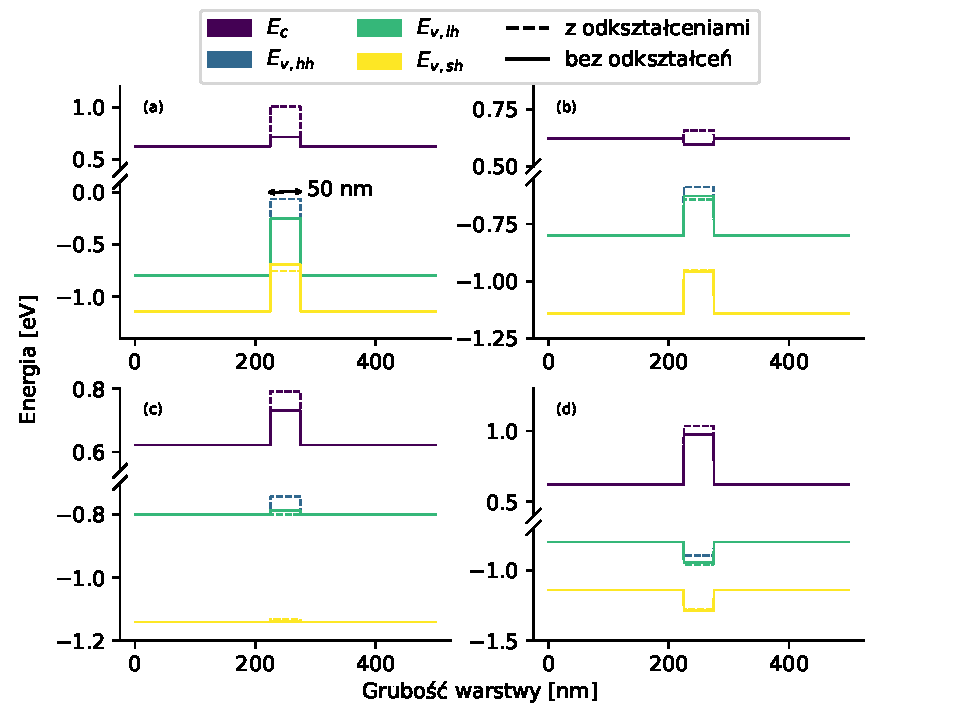
\includegraphics[width = 1\linewidth]{Figures/structure/strain_no_strain.pdf}
	\caption{Porównanie profili energetycznych badanej struktury bez uwzględnienia
	naprężeń oraz z odkształceniami. Przyjęto temperaturę \(T = 300\;[K]\).
	Składy materiału B: \\(a) \BPChem{Al\_{0.1}Ga\_{0.9}As\_{0.5}Sb\_{0.5}},
	(b) \BPChem{GaAs\_{0.9}Sb\_{0.1}}, (c) \BPChem{Al\_{0.2}Ga\_{0.8}As\_{0.9}Sb\_{0.1}},
	(d) \BPChem{Al\_{0.5}Ga\_{0.5}As\_{0.9}Sb\_{0.1}}}\label{fig:strain_no_strain}
\end{figure}

Na Rysunku~\ref{fig:strain_no_strain} przedstawiono wpływ odkształceń na profil energetyczny
badanej cienkiej warstwy w temperaturze \(T = 300[K]\). Uwzględnienie odkształceń prowadzi do podniesienia się pasma przewodnictwa,
oraz do rozszczepienia pasma walencyjnego na pasmo ciężkodziurowe, lekkodziurowe i rozszczepione
spin-orbitalnie. Są to wyniki zgodne z otrzymanymi w sekcji~\ref{sec:strain}.
Obserwujemy różne typy nieciągłości pasm np. Typ I na panelu (d)
oraz oraz Typ III na panelu (a) i (b). Widać również zależność typu nieciągłości
od składu.

Na Rysunku~\ref{fig:strain_temp} znajdują się profile energetyczne z odkształceniami, dla
różnych wartości temperatury. Jedyna widoczna zależność temperaturowa występuje
dla energii pasma przewodnictwa \(E_c\), która maleje wraz ze wzrostem
temperatury (por. Rysunek~\ref{fig:bands2} oraz Rysunek~\ref{fig:allE}). Pozostałe
pasma bardzo słabo zależą od temperatury i nie jest to widoczne w profilu energetycznym
struktury.


\begin{figure}[H]
	\centering
	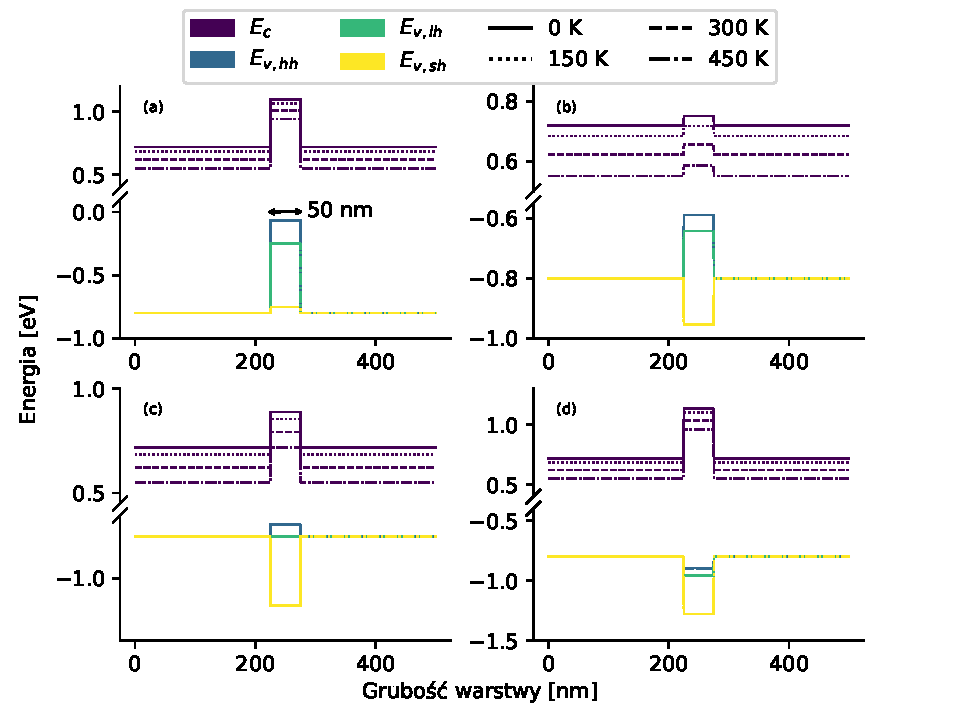
\includegraphics[width = 1\linewidth]{Figures/structure/temp_strain.pdf}
	\caption{Porównanie profili energetycznych badanej struktury ze względu na
	temperaturę. odkształcenia zostały uwzględnione.
	Składy materiału B: \\(a) \BPChem{Al\_{0.1}Ga\_{0.9}As\_{0.5}Sb\_{0.5}},
	(b) \BPChem{GaAs\_{0.9}Sb\_{0.1}}, (c) \BPChem{Al\_{0.2}Ga\_{0.8}As\_{0.9}Sb\_{0.1}},
	(d) \BPChem{Al\_{0.5}Ga\_{0.5}As\_{0.9}Sb\_{0.1}}}\label{fig:strain_temp}
\end{figure}

\section{Grubość krytyczna}

W tej części zajmiemy się oszacowaniem grubości krytycznej, jaką może osiągnąć cienka
warstwa \BPChem{Al\_{x}Ga\_{1-x}As\_{y}Sb\_{1-y}} wzrastająca na podłożu \BPChem{GaAs}.
Ponieważ między substratem a cienką warstwą występuje niedopasowanie sieciowe, komórki
elementarne materiału cienkiej warstwy są rozciągane w jednym kierunku i ściskane w drugim.
Wraz z dokładaniem kolejnych warstw materiału naprężenia rosną, aż dochodzi do powstania
pęknięcia bądź innego defektu, co prowadzi do zmniejszenia naprężeń w strukturze.
Maksymalną grubość warstwy, którą możemy osadzić na podłożu nazywamy grubością krytyczną
\(h_c\).

W celu oszacowania tej grubości posłużymy się równaniem Matthews-Blakeslee dla mieszanin
związków III-V:
\begin{equation}
	h_c = \frac{b}{2\pi f} \frac{1-0.25\nu}{1+\nu}\left( \ln{\frac{h_c}{b} +1}\right)
\label{eq:matblak}
\end{equation}
Wielkości występujące w tym równaniu to:
\begin{align*}
	b &= \frac{a}{\sqrt{2}} \;\text{- wektor Burgersa}\\
	\nu &= \frac{C_{12}}{C_{11}+C_{12}} \;\text{- współczynnik Poissona}\\
	f &= \abs{\frac{a_s-a}{a}} \; \text{- odkształcenie}
\end{align*}
Parametr \(a_s\) jest stałą sieci \BPChem{GaAs} i został wzięty z tabeli~\ref{tab:binary}.
Parametry \(a\), \(C_{11}\), \(C_{12}\) to odpowiednio stała sieci oraz parametry sztywności
\BPChem{Al\_{x}Ga\_{1-x}As\_{y}Sb\_{1-y}} wyznaczone poprzez interpolacje parametrów materiałów
binarnych z tabeli~\ref{tab:binary} oraz~\ref{tab:strain_params}.

Równanie~\ref{eq:matblak} jest nieliniowym, uwikłanym równaniem i nie możemy znaleźć analitycznego
rozwiązania. W celu jego numerycznego rozwiązania przedstawimy je w postaci:
\begin{equation}
	f(h_c) = \frac{b}{2\pi f} \frac{1-0.25\nu}{1+\nu}\left( \ln{\frac{h_c}{b} +1}\right) - h_c
	\label{eq:fhc}
\end{equation}
i poszukamy miejsc zerowych funkcji \(f(h_c)\). Prawdziwa grubość krytyczna znajduje się zazwyczaj
pomiędzy wyznaczoną z równania~\ref{eq:fhc} a jej dwukrotnością.

\begin{figure}[htbp]
	\centering
	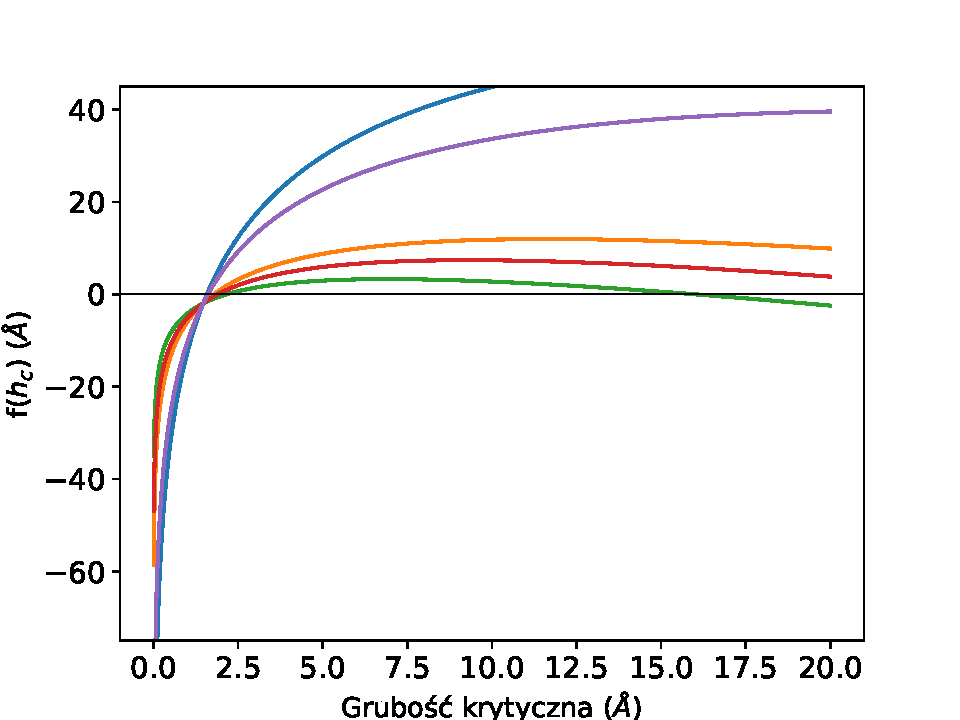
\includegraphics[width = 0.8\linewidth]{Figures/thickness/fhc.pdf}
	\caption{Wykres funkcji \(f(h_c)\) dla różnych kilku różnych zestawów parametrów.
	Po zachowaniu przebiegu funkcji widoczne są dwa miejsca zerowe. Nas będzie interesowało do drugie miejsce
	zerowe, ponieważ otrzymane z niego grubości krytyczne poprawnie przewidują wykładniczy wzrost grubości krytycznej
	wraz ze wzrostem koncentracji \BPChem{GaAs} w stopie czteroskładnikowym.}
	\label{fig:fhc}
\end{figure}

Jak widać na rysunku~\ref{fig:fhc}, funkcja \(f(h_c)\) ma prosty przebieg, i do znalezienia jej pierwiastków
nie potrzeba wyrafinowanych metod numerycznych. Dla prostoty posłużymy się implementacją w języku Python metody Brenta, będącą hybrydą metody
bisekcji, metody siecznych oraz odwrotnej interpolacji kwadratowej~\autocite{Brent1974}.

\begin{minipage}[t]{0.5\textwidth}
	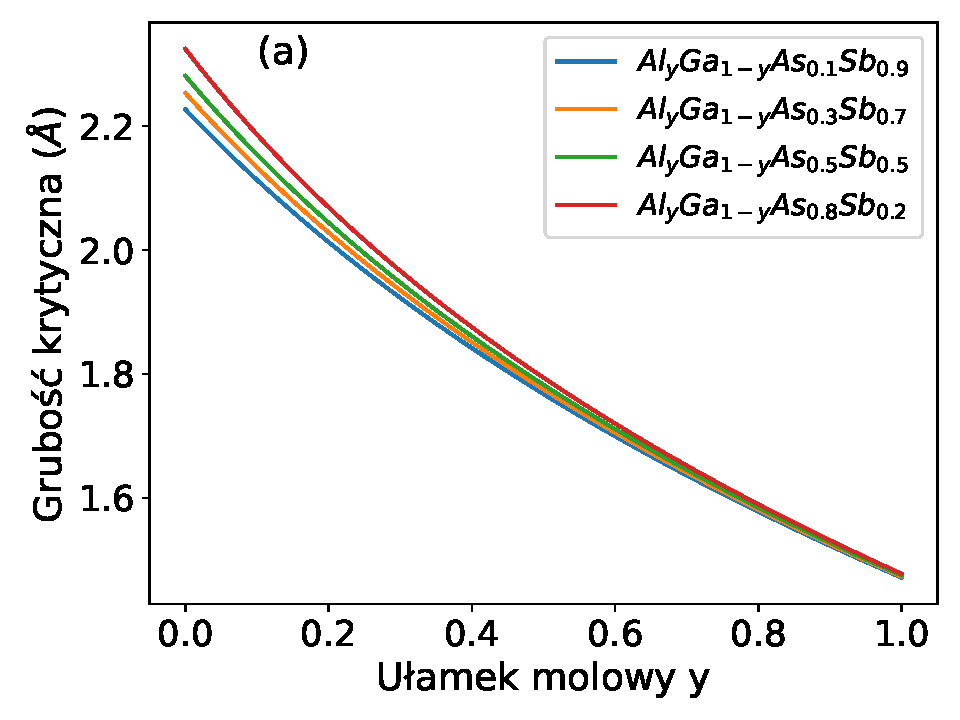
\includegraphics[width = \linewidth]{Figures/thickness/fix_x.pdf}\label{fig:hcx}
\end{minipage}
\begin{minipage}[t]{0.5\textwidth}
	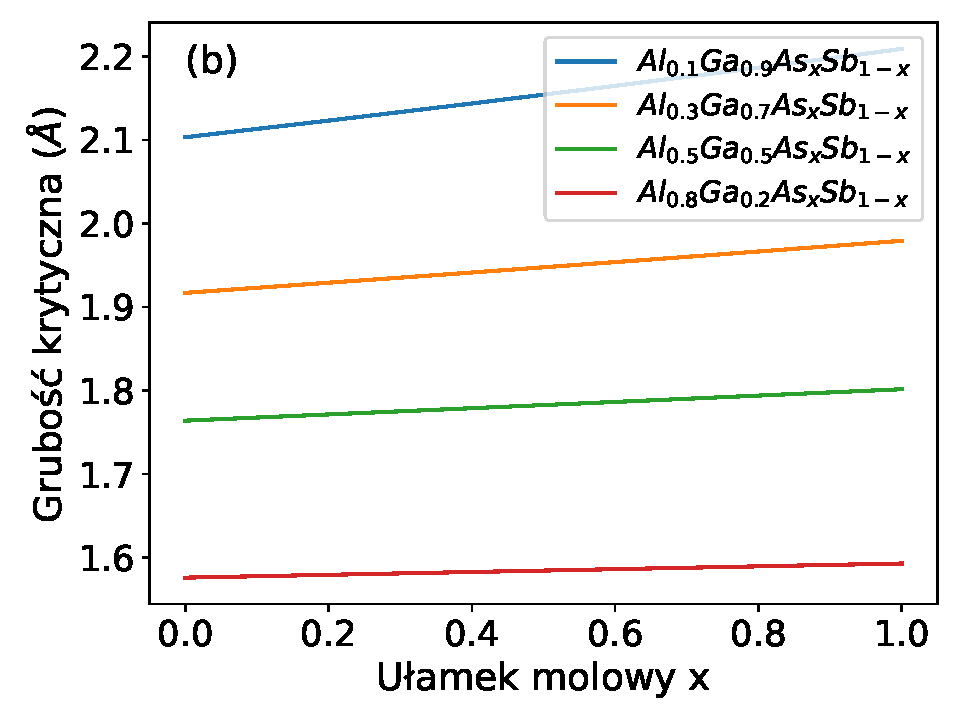
\includegraphics[width = \linewidth]{Figures/thickness/fix_y.pdf}\label{fig:hcy}
\end{minipage}
\begin{center}
\captionof{figure}{Grubości krytyczne \BPChem{Al\_{x}Ga\_{1-x}As\_{y}Sb\_{1-y}} odkładanego na podłożu \BPChem{GaAs}, w temperaturze \(T = 300K\).
Panel \((a)\) przedstawia zależność grubości krytycznej od ułamka molowego y, dla ustalonego x.
Panel \((b)\) przedstawia zależność grubości krytycznej od ułamka molowego x, dla ustalonego y.}\label{fig:hc}
\end{center}

Wyniki numerycznego poszukiwania pierwiastków równania~\ref{eq:fhc} przedstawione są 
na rysunku~\ref{fig:hc}. Widać, że czynnikiem mającym największy wpływ na grubość krytyczną jest
zawartość \BPChem{GaAs} w naszym stopie czteroskładnikowym. Jest wynik zgodny z intuicją, ponieważ
większa zawartość \BPChem{GaAs} skutkuje lepszym dopasowaniem sieciowym do podłoża i tym samym
mniejszymi naprężeniami w badanej strukturze. Ponadto, wraz ze zbliżaniem się koncentracji
\BPChem{GaAs} do jedności, grubość krytyczna rośnie do nieskończoności, co odzwierciedla fakt, że w przypadku
dobrego dopasowania sieciowego możemy nanieść bardzo grubą warstwę na podłoże.

\section{Przybliżenie paraboliczne. Struktura pasmowa i gęstość stanów.
\label{sec:parabolic}}

Teraz zajmiemy się analizą struktury pasmowej badanych materiałów, wykorzystując do tego
przybliżenie paraboliczne. Rozważamy diagonalny Hamiltonian postaci:
\begin{equation}
	\hat{H} = 
	\begin{pmatrix}
		E_c & 0 & 0 & 0\\
		0 & E_{v,hh} & 0 & 0\\
		0 & 0 & E_{v,lh} & 0\\
		0 & 0 & 0 & E_{v,sh}
	\end{pmatrix}
	\label{eq:hamiltonian}
\end{equation}

gdzie elementy diagonalne mają postać:
\begin{align}
	&E_c = E_v + E_g + E_{c,k} + \delta E_{c,a}\\
	&E_{v,hh} = E_v - E_{hh,k} + \delta E_{v,a} - \delta E_{b,v}\\
	&E_{v,lh} = E_v - E_{lh,k} + \delta E_{v,a} + \delta E_{b,v}^{+}\\
	&E_{v,sh} = E_v - E_{sh,k} + \delta E_{v,a} + \delta E_{b,v}^{-}
\end{align}

Wielkości występujące w powyższych równaniach zostały zdefiniowane w~\eqref{eq:strains}.
Dodatkowo pojawiła się wielkość \(E_{i,k}\), zdefiniowana wzorem:
\begin{equation}
	E_{i,k} = \frac{\hbar^2 k^2}{2 m_0} \frac{1}{m_i}
	\label{eq:parabolic}
\end{equation}
gdzie \(m_i\) jest masą efektywną elektronu/dziury. Interesuje nas struktura pasmowa na kierunku \([0 0 1]\).
Masy efektywne na tym kierunku wyrażone są poprzez liniowe kombinacje parametrów Luttingera:
\begin{align*}
	&m_c = m_c^{\ast}\\
	&m_{hh} = \frac{1}{\gamma_1 - 2\gamma_2}\\
	&m_{lh} = \frac{1}{\gamma_1 + 2\gamma_2}\\
	&m_{sh} = \frac{1}{\gamma_1}
\end{align*}

\(m_c^{\ast}\) to masa efektywna w paśmie przewodnictwa, policzona przy pomocy schematu interpolacyjnego.

\begin{table}[htbp]
	\centering
\caption{Parametry Luttingera materiałów binarnych~\autocite{Vurgaftman2001}.}
\begin{tabular}{ccccc}
	\toprule
	\toprule
	Parametr & \BPChem{AlAs} & \BPChem{AlSb} &  \BPChem{GaSb} & \BPChem{GaAs}\\
	\midrule
	\(\gamma_1\)     	& 3.76 & 5.18  & 13.4 & 6.98 \\
	\(\gamma_2\)     	& 0.82 & 1.19  & 4.7  & 2.06 \\
\bottomrule
  \bottomrule  
  \end{tabular}%
	\label{tab:luttinger}%
  \end{table}%

Parametry Luttingera dla materiału czteroskładnikowy zostały otrzymane przy pomocy
schematu interpolacyjnego, opisanego w~\ref{sec:interpolation}.

Przeanalizujemy również, jak wygląda gęstość stanów w rozważanym przybliżeniu parabolicznym.
Jest ona dana wzorem:
\begin{equation}
	D_{i}(E) = \frac{1}{2\pi^2}\left(2\frac{m_{DOS}^i}{hbar^2}\right)^{\frac{3}{2}} \left(E-E_i\right)^{\frac{1}{2}}
	\label{eq:DOS}
\end{equation}
Masy efektywne \(m_{DOS}^{i}\) są interpolowanymi masami z Tabeli~\ref{tab:binary}.
Poniżej przedstawione zostały wykresy struktur pasmowych oraz gęstości stanów dla materiałów binarnych.


\begin{minipage}[t]{0.5\textwidth}
	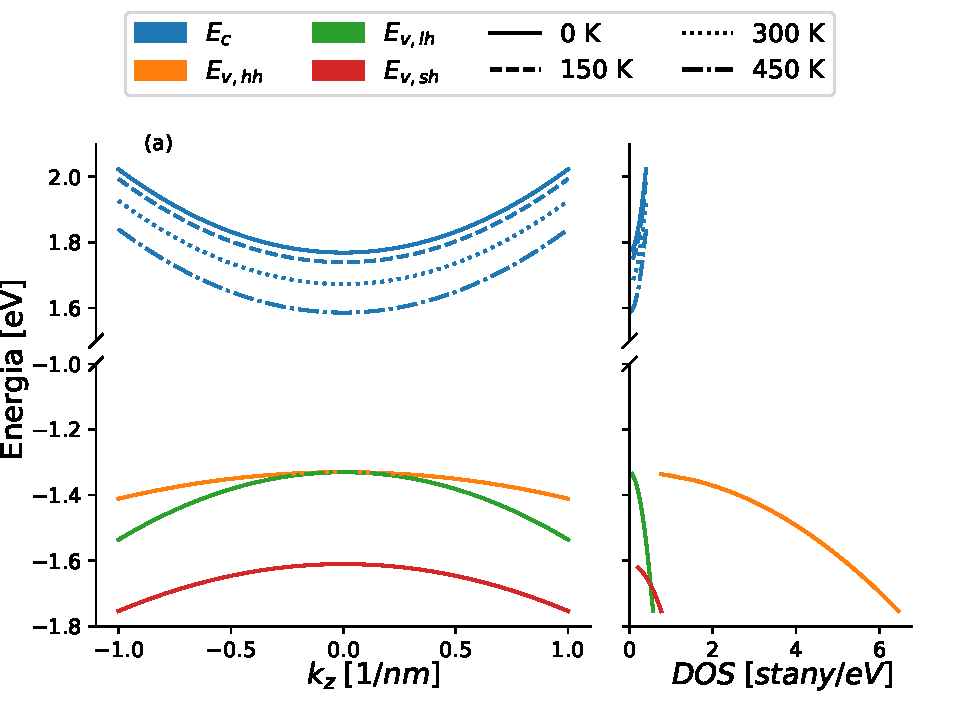
\includegraphics[width = 1.05\linewidth]{Figures/band_str/AlAs.pdf}\label{fig:AlAs_bs}
\end{minipage}
\begin{minipage}[t]{0.5\textwidth}
	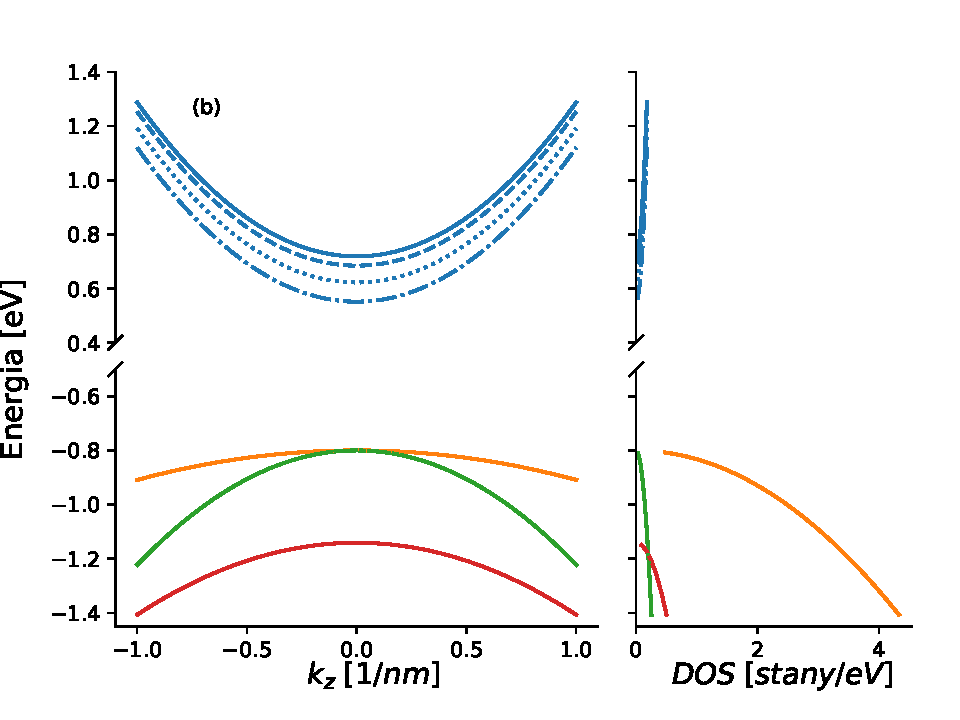
\includegraphics[width = 1.05\linewidth]{Figures/band_str/GaAs.pdf}\label{fig:GaAs_bs}
\end{minipage}
\begin{minipage}[t]{0.5\textwidth}
	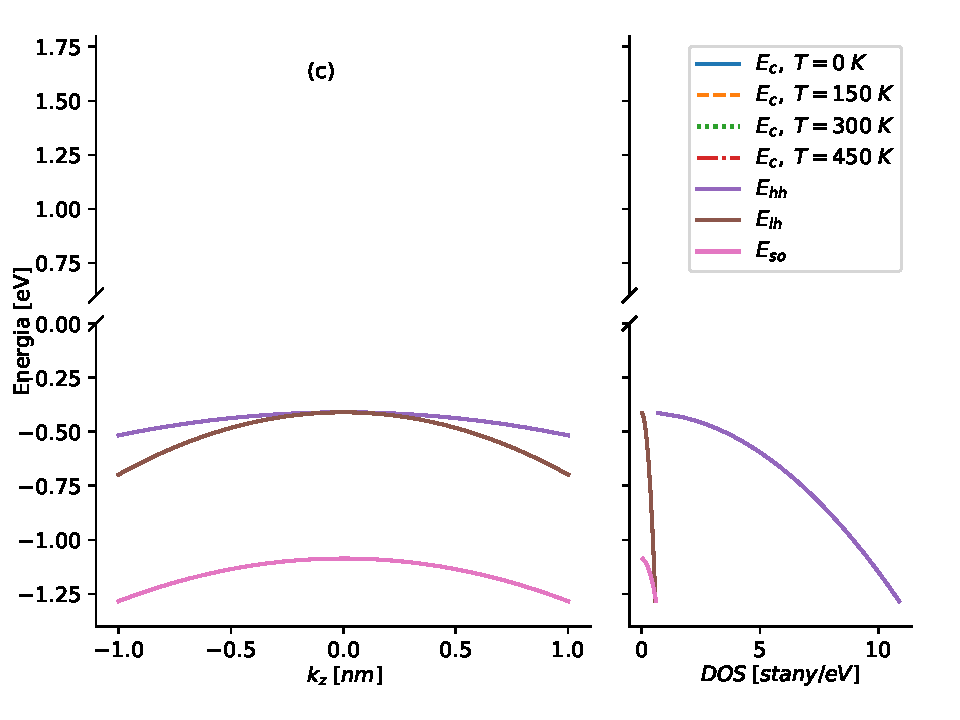
\includegraphics[width = 1.05\linewidth]{Figures/band_str/AlSb.pdf}\label{fig:AlSb_bs}
\end{minipage}
\begin{minipage}[t]{0.5\textwidth}
	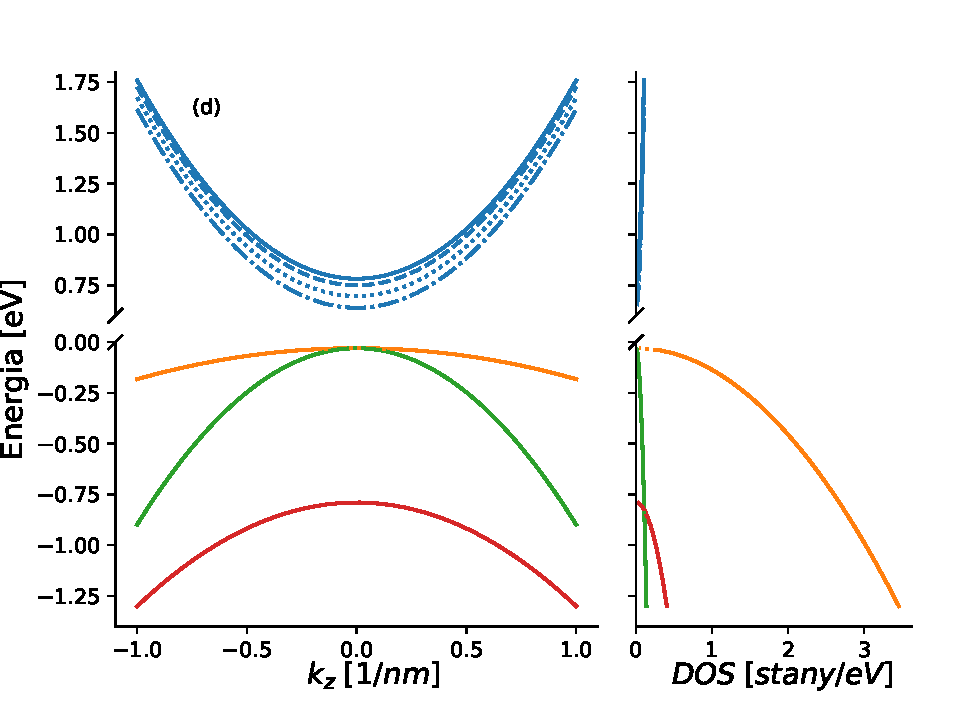
\includegraphics[width = 1.05\linewidth]{Figures/band_str/GaSb.pdf}\label{fig:GaSb_bs}
\end{minipage}
\begin{center}
	\captionof{figure}{Struktury pasmowe oraz gęstości stanów materiałów binarnych. (a) \BPChem{AlAs}, 
	(b) \BPChem{GaAs}, (c) \BPChem{AlSb}, (d) \BPChem{GaSb}}
\end{center}

W następnej kolejności chcemy przeanalizować zależność struktury pasmowej
materiału czteroskładnikowego na podłożu \BPChem{GaAs} od składu oraz odkształceń.

\begin{minipage}[t]{0.5\textwidth}
	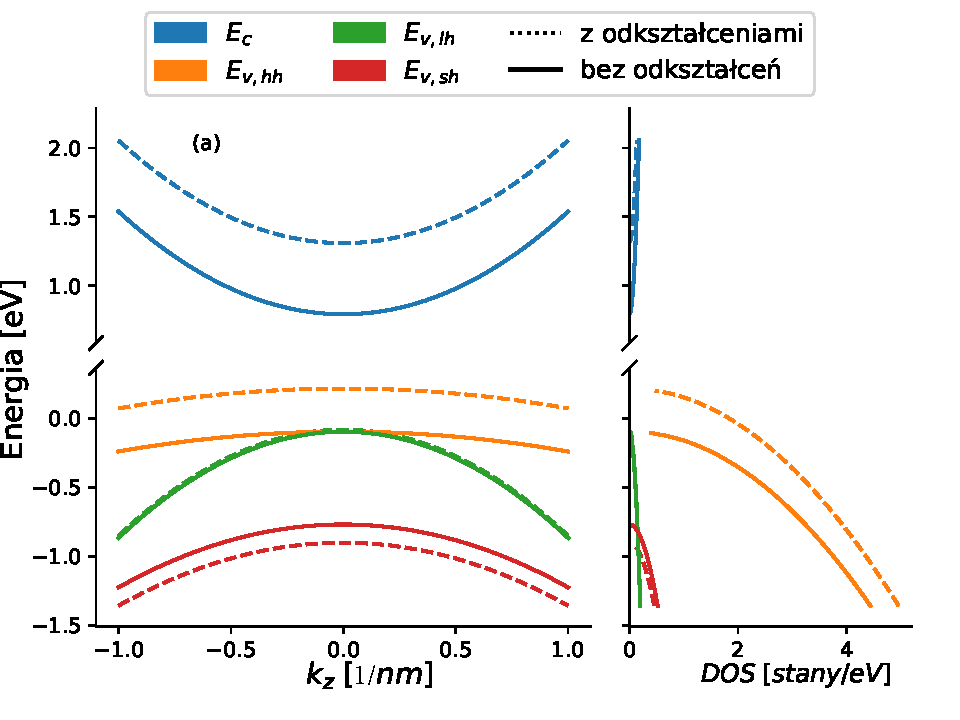
\includegraphics[width = 1.05\linewidth]{Figures/band_str/good/ns_x_0.1_y_0.1.pdf}\label{fig:bs_x_0.1_y_0.1_ns}
\end{minipage}
\begin{minipage}[t]{0.5\textwidth}
	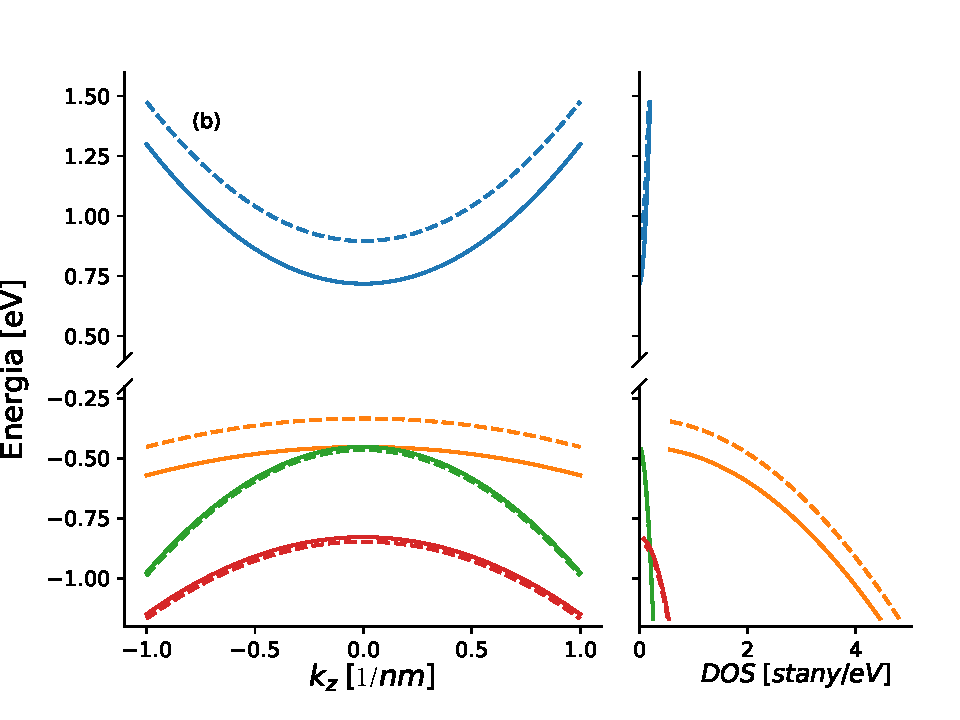
\includegraphics[width = 1.05\linewidth]{Figures/band_str/good/ns_x_0.1_y_0.7.pdf}\label{fig:bs_x_0.1_y_0.7_ns}
\end{minipage}
\begin{minipage}[t]{0.5\textwidth}
	\includegraphics[width = 1.05\linewidth]{Figures/band_str/good/ns_x_0.5_y_0.1.pdf}\label{fig:bs_x_0.5_y_0.1_ns}
\end{minipage}
\begin{minipage}[t]{0.5\textwidth}
	\includegraphics[width = 1.05\linewidth]{Figures/band_str/good/ns_x_0.9_y_0.5.pdf}\label{fig:bs_x_0.9_y_0.5_ns}
\end{minipage}
\begin{center}
	\captionof{figure}{Struktury pasmowe oraz gęstości stanów materiału czteroskładnikowego. Odkształcenia dla temperatury
	\(T = 300\; K\). \\(a) \BPChem{Al\_{0.1}Ga\_{0.9}As\_{0.1}Sb\_{0.9}},
	(b) \BPChem{Al\_{0.1}Ga\_{0.9}As\_{0.7}Sb\_{0.3}}, (c) \BPChem{Al\_{0.5}Ga\_{0.5}As\_{0.1}Sb\_{0.9}},
	(d) \BPChem{Al\_{0.9}Ga\_{0.1}As\_{0.5}Sb\_{0.5}}}
\end{center}

Największy wpływ odkształcenia mają na pasmo przewodnictwa, oraz walencyjne pasmo
ciężkodziurowe. Jest to zgodne z poprzednimi wynikami - patrz Rysunek~\ref{fig:strain_no_strain}.

\begin{minipage}[t]{0.5\textwidth}
	\includegraphics[width = 1.05\linewidth]{Figures/band_str/good/x_0.1_y_0.3.pdf}\label{fig:bs_x_0.1_y_0.3}
\end{minipage}
\begin{minipage}[t]{0.5\textwidth}
	\includegraphics[width = 1.05\linewidth]{Figures/band_str/good/x_0.1_y_0.9.pdf}\label{fig:bs_x_0.1_y_0.9}
\end{minipage}
\begin{minipage}[t]{0.5\textwidth}
	\includegraphics[width = 1.05\linewidth]{Figures/band_str/good/x_0.5_y_0.9.pdf}\label{fig:bs_x_0.5_y_0.9}
\end{minipage}
\begin{minipage}[t]{0.5\textwidth}
	\includegraphics[width = 1.05\linewidth]{Figures/band_str/good/x_0.9_y_0.5.pdf}\label{fig:bs_x_0.9_y_0.5}
\end{minipage}
\begin{center}
	\captionof{figure}{Struktury pasmowe oraz gęstości stanów materiału czteroskładnikowego, z uwzględnieniem
	odkształceń temperaturowych.
	 \\(a) \BPChem{Al\_{0.1}Ga\_{0.9}As\_{0.3}Sb\_{0.7}},
	(b) \BPChem{Al\_{0.1}Ga\_{0.9}As\_{0.9}Sb\_{0.1}}, (c) \BPChem{Al\_{0.5}Ga\_{0.5}As\_{0.9}Sb\_{0.1}},
	(d) \BPChem{Al\_{0.9}Ga\_{0.1}As\_{0.5}Sb\_{0.5}}}
	\label{fig:bs}
\end{center}

Zmiana temperatury ma największy wpływ na pasmo przewodnictwa. Jest to wynik oczekiwany, ponieważ
temperatura słabo wpływa na zmianę energii, a w paśmie przewodnictwa uwzględniona jest przerwa energetyczna,
która zależy od temperatury poprzez równanie~\eqref{eq:varshi}.

Gęstości stanów zależą od odkształceń jakościowo podobnie do odpowiadających im pasm energetycznych. Największe
wartości gęstość stanów przyjmuje dla ciężkich dziur, ponieważ mają one największą masę efektywną, a gęstość stanów
zależy od niej potęgowo.

Lokalna gęstość stanów bierze pod uwagę niejednorodności próbki, czyli zależność gęstości elektronowej od położenia
wewnątrz próbki. W naszych obliczeniach zakładamy jednorodność próbki, więc gęstość stanów przyjmuje takie same wartości
w każdym jej miejscu.

\newpage


\section{Gęstość nośników}

Gęstość nośników określa ilość nośników ładunku na jednostkę objętości i zazwyczaj podawana jest
jako wartość średnia na obszarze całego materiału. Jest to istotna wielkość, występująca w równaniach
dotyczących przewodnictwa elektrycznego i termicznego. Teoretycznie można ją wyznaczyć poprzez całkowanie
gęstości stanów z funkcją rozkładu Fermiego-Diraca:

\begin{equation}
	f\left(E\right) = \frac{1}{1+e^{\frac{E-E_F}{k_b T}}}
	\label{eq:FD}
\end{equation}

W obliczeniach posługujemy się prostym przybliżeniem
parabolicznym, więc gęstość stanów jest dana równaniem~\eqref{eq:DOS}.
Badamy heterostrukturę \BPChem{GaAs}\(\backslash\)\BPChem{Al\_{x}Ga\_{1-x}As\_{y}Sb\_{1-y}}\(\backslash\)\BPChem{GaAs},
złożoną z dwóch warstw \BPChem{GaAs} o grubości \(500\;nm\) oraz warstwy \BPChem{Al\_{x}Ga\_{1-x}As\_{y}Sb\_{1-y}}
pomiędzy nimi. Grubość centralnej warstwy zmienia się od \(100\;nm\) do \(500\;nm\).
Dla uproszczenia ustalamy \(y = 0.9\) i będziemy zmieniali tylko \(x\).
W celu wyznaczenia średniej gęstości stanów w heterostrukturze posłużymy się średnią ważoną, za wagi przyjmując
grubości poszczególnych warstw. Wzór na średnią gęstość stanów przyjmuje postać:
\begin{equation}
	D_i= \frac{2\cdot D_i^{\BPChem{GaAs}}\cdot d_{\BPChem{GaAs}} +
	 D_i^{\BPChem{AlGaAsSb}} \cdot d_{\BPChem{AlGaAsSb}} }{2\cdot d_{\BPChem{GaAs}}+d_{\BPChem{AlGaAsSb}}}
\end{equation}

\begin{figure}[h]
	\centering
	\includegraphics[width=0.7\textwidth]{Figures/carriers/integrand.pdf}
	\caption{Poglądowy rysunek przedstawiający gęstość stanów w paśmie przewodnictwa, rozkład
	Fermiego-Diraca oraz ich iloczyn. Pole zacieniowanego obszaru to szukana koncentracja elektronów,
	dana równaniem~\eqref{eq:n_conc}.}
	\label{<label>}
\end{figure}

\noindent Gęstość elektronów wyznaczymy więc ze wzoru:
\begin{equation}
	n = \int_{E_c}^{\infty}D_{c}(E)f(E)\,dx
	\label{eq:n_conc} 
\end{equation}
gdzie \(E_c = \min{\{E_c^{\BPChem{GaAs}},E_c^{\BPChem{AlGaAsSb}}\}}\) czyli jest krawędzią pasma przewodnictwa. 
Natomiast gęstość dziur możemy policzyć ze wzoru:
\begin{equation}
	p = \int_{-\infty}^{E_v}\left(D_{lh}(E)+D_{hh}(E)\right)\left(1-f(E)\right)\,dx
	\label{eq:p_conc}
\end{equation}
gdzie \(E_v\) jest największa wartością spośród krawędzi pasm walencyjnych. Funkcja rozkładu
dla dziur ma postać:
\begin{equation}
	1-f(E) = 1 - \frac{1}{1+e^{\frac{E-E_F}{k_b T}}} = \frac{1}{1+e^{\frac{-E+E_F}{k_b T}}}
	\label{eq:FD_holes}
\end{equation}



Interesującą nas koncentracje elektronów oraz dziur wyznaczymy wykonując
całki~\eqref{eq:n_conc} oraz~\eqref{eq:p_conc} numerycznie. Innym podejściem
jest przybliżenie rozkładu Fermiego-Diraca poprzez klasyczny rozkład Maxwella-Boltzmanna
(przybliżenie to jest słuszne dla \(|E-E_f|\gg k_b T\), co jest spełnione dla półprzewodników w
pobliżu temperatury pokojowej). Pozwala to na przeprowadzenie całkowania w sposób
analityczny i prowadzi do wyników:
\begin{align}
	n&\sim \exp\left(-\frac{E_c-E_F}{k_b T}\right)\\\nonumber
	p&\sim \exp\left(-\frac{E_F-E_v}{k_b T}\right)\\
	\label{eq:approx}
\end{align}
Przybliżenia te pozwolą na zweryfikowanie poprawności numerycznego całkowania.

A priori nie znamy położenia poziomu Fermiego potrzebnego do wyznaczenia funkcji rozkładu.
Możemy jednak wykreślić w jaki sposób zmieniają się koncentrację nośników wraz z jego położeniem.


\begin{minipage}[t]{0.5\textwidth}
	\hspace{-0.54cm}
	\includegraphics[width = \linewidth]{Figures/carriers/concentration_L_100.pdf}
\end{minipage}
\begin{minipage}[t]{0.5\textwidth}
	\hspace{-0.54cm}
	\includegraphics[width = 1.0\linewidth]{Figures/carriers/concentration_L_200.pdf}
\end{minipage}
\begin{minipage}[t]{0.5\textwidth}
	\includegraphics[width = 1.0\linewidth]{Figures/carriers/concentration_L_400.pdf}
\end{minipage}
\begin{minipage}[t]{0.5\textwidth}
	\includegraphics[width = 1.0\linewidth]{Figures/carriers/concentration_L_500.pdf}
\end{minipage}
\begin{center}
	\captionof{figure}{Zależność koncentracji nośników od położenia poziomu Fermiego w \(T = 300\;K\).
	Poziom Fermiego jest przesunięty tak, by wartość 0 eV odpowiadała VBO.
	Linią ciągłą narysowana jest koncentracja elektronów, a linią przerywaną koncentracja dziur z pasma lekko-
	i ciężkodziurowego. Kolejne panele przedstawiają różne grubości warstwy \BPChem{AlGaAsSb}:
	(a) 100 nm, (b) 200 nm, (c) 400 nm, (d) 500 nm. }
	\label{fig:conc}
\end{center}

Na wykresie~\ref{fig:conc} widzimy, że w skali logarytmicznej koncentracje nośników są liniowymi
funkcjami poziomu Fermiego. Jest to zgodne z wzorami~\eqref{eq:approx}.
Łatwo zauważyć, że wraz ze wzrostem grubości rośnie koncentracja dziur. 
Prawdopodobnie dzieje się tak, ponieważ gęstość stanów w paśmie walencyjnym materiału czteroskładnikowego
jest większa niż w \BPChem{GaAs}, a wraz ze wzrostem grubości warstwy \BPChem{AlGaAsSb} rośnie jej
wkład do średniej gęstości stanów (por. rysunki w sekcji~\ref{sec:parabolic}). Dokładne zależności
gęstości stanów od grubości warstwy oraz składu przedstawione są w \hyperref[chapt:dodatek2]{Dodatku 2}.
Wraz ze wzrostem ułamka molowego \(x\) (stopniowym przechodzeniem od
\BPChem{GaAs\_{0.9}Sb\_{0.1}} do \BPChem{AlAs\_{0.9}Sb\_{0.1}}) rośnie koncentracja dziur a maleje koncentracja
elektronów. Ten wzrost spowalnia wraz ze wzrostem grubości cienkiej warstwy.

Koncentracje dziur oraz elektronów przecinają się w dokładnie jednym miejscu. Oznacza to, że
istnieje takie \(E_F\) dla którego \(n = p\). Jest to tzw. warunek równowagi elektrycznej i wykorzystamy
go do systematycznego wyznaczenia wartości poziomu Fermiego, dla którego osiągana jest równowaga
w danej temperaturze. W tym celu będziemy szukali miejsce zerowych funkcji 
\(g(E_F) = n(E_F) - p(E_F)\) w ustalonej temperaturze. Posłużymy się znaną już metodą Brenta~\autocite{Brent1974}.



\begin{minipage}[t]{0.5\textwidth}
	\hspace{-0.54cm}
	\includegraphics[width = \linewidth]{Figures/carriers/fermi_L_100.pdf}
\end{minipage}
\begin{minipage}[t]{0.5\textwidth}
	\hspace{-0.54cm}
	\includegraphics[width = \linewidth]{Figures/carriers/fermi_L_200.pdf}
\end{minipage}
\begin{minipage}[t]{0.5\textwidth}
	\includegraphics[width = \linewidth]{Figures/carriers/fermi_L_400.pdf}
\end{minipage}
\begin{minipage}[t]{0.5\textwidth}
	\includegraphics[width = \linewidth]{Figures/carriers/fermi_L_500.pdf}
\end{minipage}
\begin{center}
	\captionof{figure}{Zależność temperaturowa poziomu Fermiego oraz koncentracji nośników w równowadze
	elektrycznej. Kolejne pary paneli przedstawiają różne grubości warstwy \BPChem{AlGaAsSb}:
	(a) 100 nm, (b) 200 nm, (c) 400 nm, (d) 500 nm. }
	\label{fig:ef}
\end{center}

Na rysunku~\ref{fig:ef} widzimy, że poziom Fermiego maleje wraz z temperaturą. Z kolei
zmiana grubości cienkiej warstwy powoduje zmniejszenie nachylenia poziomu Fermiego w funkcji
temperatury. Zmieniając ułamek molowy \(x\) na zakresie od 0 do 1 poziom Fermiego
rośnie, co jest zgodne z~\ref{fig:conc}. Największe różnice
widoczne są pomiędzy jego małymi wartościami. Dla \(x\gtrapprox 0.5\) nie obserwujemy znaczących
zmian wraz z dalszym wzrostem ułamka molowego.

% \chapter{Wyniki i dyskusja}\label{chapt:results}


\chapter*{Dodatek 1: Wykresy parametrów materiałów trójskładnikowych}\label{chapt:dodatek}
\addcontentsline{toc}{chapter}{Dodatek 1: Wykresy parametrów materiałów trójskładnikowych}
Poniżej zostały przestawione wykresy interesujących nas parametrów:


\begin{minipage}[t]{0.5\textwidth}
	\includegraphics[width = \linewidth]{Figures/ternary/eg.pdf}\label{fig:ter_Eg}
\end{minipage}
\begin{minipage}[t]{0.5\textwidth}
	\includegraphics[width = \linewidth]{Figures/ternary/vbo.pdf}\label{fig:ter_vbo}
\end{minipage}

\begin{minipage}[t]{0.5\textwidth}
	\includegraphics[width = \linewidth]{Figures/ternary/delta_so.pdf}\label{fig:ter_delta_so}
\end{minipage}
\begin{minipage}[t]{0.5\textwidth}
	\includegraphics[width = \linewidth]{Figures/ternary/alc.pdf}\label{fig:ter_alc}
\end{minipage}

\begin{minipage}[t]{0.5\textwidth}
	\includegraphics[width = \linewidth]{Figures/ternary/m_e.pdf}\label{fig:ter_me}
\end{minipage}
\begin{minipage}[t]{0.5\textwidth}
	\includegraphics[width = \linewidth]{Figures/ternary/m_hh.pdf}\label{fig:ter_mhh}
\end{minipage}

\begin{center}
\begin{minipage}[t]{0.5\textwidth}
	\includegraphics[width = \linewidth]{Figures/ternary/m_lh.pdf}\label{fig:ter_mlh}
\end{minipage}
\captionof{figure}{Wykresy parametrów stopów trójskładnikowych w funkcji ułamka molowego \(x\).}
\end{center}

\chapter*{Dodatek 2: Zależność gęstości stanów od składu i grubości cienkiej warstwy}\label{chapt:dodatek2}
\addcontentsline{toc}{chapter}{Dodatek 2: Zależność gęstości stanów od składu i grubości cienkiej warstwy}


\begin{minipage}[t]{0.42\textwidth}
	\hspace{-2.1cm}
	\includegraphics[width = 1\linewidth]{Figures/carriers/dos_L_100.pdf}
\end{minipage}
\begin{minipage}[t]{0.42\textwidth}
	\hspace{-2.5cm}
	\includegraphics[width = 1\linewidth]{Figures/carriers/dos_L_300.pdf}
\end{minipage}
\begin{minipage}[t]{0.42\textwidth}
	\hspace{-2.7cm}
	\includegraphics[width = 1\linewidth]{Figures/carriers/dos_L_500.pdf}
\end{minipage}
\begin{minipage}[t]{0.4\textwidth}
	\hspace{-1.5cm}
	\includegraphics[width = \linewidth]{Figures/carriers/dos_val_L_100.pdf}
\end{minipage}
\begin{minipage}[t]{0.4\textwidth}
	\hspace{-1.5cm}
	\includegraphics[width = \linewidth]{Figures/carriers/dos_val_L_300.pdf}
\end{minipage}
\begin{minipage}[t]{0.4\textwidth}
	\hspace{-1.5cm}
	\includegraphics[width = \linewidth]{Figures/carriers/dos_val_L_500.pdf}
\end{minipage}
\begin{center}
	\captionof{figure}{Zależność gęstości stanów od składu oraz grubości cienkiej warstwy.
	Pierwszy rząd przedstawia gęstość stanów w paśmie przewodnictwa dla grubości: (a) 100 nm,
	(b) 300 nm, (c) 500 nm. Drugi rząd przedstawia gęstość stanów w paśmie 
	walencyjnym dla grubości: (d) 100 nm, (e) 300 nm, (f) 500 nm.}
	\label{fig:dos_d}
\end{center}

	
	% Adding a bibliography if citations are used in the report
	% Un/Comment the following line to customize the Bibliography title
	\renewcommand{\bibname}{Bibliografia}
	
	% \bibliography{AlGaAsSb.bib}
	
	% Uncomment the following two lines to remvoe the cc license
	% \vspace*{\fill}
	% {\hypersetup{urlcolor=black}{\scriptsize \doclicenseThis}}
	% Adds reference to the Bibliography in the ToC
	\addcontentsline{toc}{chapter}{\bibname}
	\printbibliography{}
	 \pagebreak
	
	
		

\end{document}